%% Version 6.1, 1 September 2021
%
%%%%%%%%%%%%%%%%%%%%%%%%%%%%%%%%%%%%%%%%%%%%%%%%%%%%%%%%%%%%%%%%%%%%%%
% TemplateV6.1.tex --  LaTeX-based blank template for submissions to the 
% American Meteorological Society
%
%%%%%%%%%%%%%%%%%%%%%%%%%%%%%%%%%%%%%%%%%%%%%%%%%%%%%%%%%%%%%%%%%%%%%
% PREAMBLE
%%%%%%%%%%%%%%%%%%%%%%%%%%%%%%%%%%%%%%%%%%%%%%%%%%%%%%%%%%%%%%%%%%%%%

%% Start with one of the following:
% 1.5-SPACED VERSION FOR SUBMISSION TO THE AMS
\documentclass{ametsocV6.1}

% TWO-COLUMN JOURNAL PAGE LAYOUT---FOR AUTHOR USE ONLY
% \documentclass[twocol]{ametsocV6.1}

%%%%%%%%%%%%%%%%%%%%%%%%%%%%%%%%

%%% To be entered by author:

%% May use \\ to break lines in title:

\title{Understanding Predictability of Daily Southeast US Precipitation using Explainable Machine Learning}

%% Enter authors' names and affiliations as you see in the examples below.
%
%% Use \correspondingauthor{} and \thanks{} (\thanks command to be used for affiliations footnotes, 
%% such as current affiliation, additional affiliation, deceased, co-first authors, etc.)
%% immediately following the appropriate author.
%
%% Note that the \correspondingauthor{} command is NECESSARY.
%% The \thanks{} commands are OPTIONAL.
%
%% Enter affiliations within the \affiliation{} field. Use \aff{#} to indicate the affiliation letter at both the
%% affiliation and at each author's name. Use \\ to insert line breaks to place each affiliation on its own line.

%\authors{Author One,\aff{a}\correspondingauthor{Author One, email@email.com} 
%Author Two,\aff{a} 
%Author Three,\aff{b} 
%Author Four,\aff{a} 
%Author Five\thanks{Author Five's current affiliation: NCAR, Boulder, Colorado},\aff{c} 
%Author Six,\aff{c} 
%Author Seven,\aff{d}
% and Author Eight\aff{a,d}
%}
%
%\affiliation{\aff{a}{First Affiliation}\\
%\aff{b}{Second Affiliation}\\
%\aff{c}{Third Affiliation}\\
%\aff{d}{Fourth Affiliation}
%}

\authors{Kathy Pegion\aff{a},\correspondingauthor{Kathy Pegion, kpegion@gmu.edu}
Emily J. Becker,\aff{b} 
Ben P. Kirtman\aff{b} 
}

\affiliation{\aff{a}{George Mason University, Department of Atmospheric, Oceanic, and Earth Sciences, Fairfax, VA}\\
\aff{b}{University of Miami/RSMAS/CIMAS, Miami, FL}
}

%%%%%%%%%%%%%%%%%%%%%%%%%%%%%%%%%%%%%%%%%%%%%%%%%%%%%%%%%%%%%%%%%%%%%
% ABSTRACT
%
% Enter your abstract here
% Abstracts should not exceed 250 words in length!
%
 
\abstract{We investigate the predictability of the sign of daily South-East US (SEUS) precipitation anomalies associated with large-scale climate variability where the predictors are perfectly known using machine learning models.  Indices of climate phenomena (e.g., NAO, AMO, PDO, ENSO, MJO, etc.) produce neither accurate nor reliable predictions, indicating that the indices themselves are not good predictors.  A convolutional neural network using gridded fields as predictors is reliable and more accurate than the index based models.  Using explainable machine learning we identify which variables and gridpoints of the input fields are most relevant for confident and correct predictions.  Our results show that the local circulation is most important as represented by maximum relevance of 850hPa geopotential heights and zonal winds to making skillful, high probability predictions.  Corresponding composite anomalies identify connections with the El-Ni\~{n}o Southern Oscillation during winter and the Atlantic Multidecadal Oscillation and North American Subtropical High during summer.}

\begin{document}

%% Necessary!
\maketitle

%%%%%%%%%%%%%%%%%%%%%%%%%%%%%%%%%%%%%%%%%%%%%%%%%%%%%%%%%%%%%%%%%%%%%
% SIGNIFICANCE STATEMENT/CAPSULE SUMMARY
%%%%%%%%%%%%%%%%%%%%%%%%%%%%%%%%%%%%%%%%%%%%%%%%%%%%%%%%%%%%%%%%%%%%%
%
% If you are including an optional significance statement for a journal article or a required capsule summary for BAMS 
% (see www.ametsoc.org/ams/index.cfm/publications/authors/journal-and-bams-authors/formatting-and-manuscript-components for details), 
% please apply the necessary command as shown below:
%
% Significance Statement (all journals except BAMS)
%
%\statement
%	 Enter significance statement here, no more than 120 words. See \url{www.ametsoc.org/index.cfm/ams/publications/author-information/significance-statements/} for details.
%
%% Capsule (BAMS only)
%%
%\capsule
%       Enter BAMS capsule here, no more than 30 words. See \url{www.ametsoc.org/index.cfm/ams/publications/author-information/formatting-and-manuscript-components/#capsule} for details.
%
%% * * If using twocol mode, you will need to use the commands "twocolsig" and "twocolcapsule" in place of "sig" and "capsule"
%%      to ensure that the text box correctly spans across both columns.
%

%%%%%%%%%%%%%%%%%%%%%%%%%%%%%%%%%%%%%%%%%%%%%%%%%%%%%%%%%%%%%%%%%%%%%
% MAIN BODY OF PAPER
%%%%%%%%%%%%%%%%%%%%%%%%%%%%%%%%%%%%%%%%%%%%%%%%%%%%%%%%%%%%%%%%%%%%%
%

%% In all cases, if there is only one entry of this type within
%% the higher level heading, use the star form: 
%%
% \section{Section title}
% \subsection*{subsection}
% text...
% \section{Section title}

%vs

% \section{Section title}
% \subsection{subsection one}
% text...
% \subsection{subsection two}
% \section{Section title}

%%%
% \section{First primary heading}

% \subsection{First secondary heading}

% \subsubsection{First tertiary heading}

% \paragraph{First quaternary heading}

\section{Introduction}
\label{sec:intro}

Predicting when, where, and how much precipitation will fall is critical for decision-making and responding to the impacts of extreme rainfall across a wide range of sectors and timescales \citep{DOE:2020}. The predictability of subseasonal-to-seasonal (S2S) precipitation stems from many different sources, varies by season, and is changing with anthropogenic climate change \citep{DOE:2020}. S2S prediction of total precipitation, particularly in the extra-tropics and during the warm season by state-of-the-art coupled Earth system models (ESMs) is overall quite poor, as the current generation of ESMs have large biases that profoundly limit the ability to simulate and predict the circulation patterns that lead to much of the spatial-temporal variability of precipitation \citep{DOE:2020}. 

The skill of predicting even total weekly and monthly precipitation anomalies over North America remains poor \citep[e.g.,][]{pegion_subseasonal_2019,becker_evolution_2020}. To add to the challenge, actionable predictions require the ability to predict precipitation and its extremes at higher temporal resolution and at regional scales. Prolonged dry spells or the rains from a single event can have devastating impacts.   

In particular, S2S precipitation variability in the Southeastern United States (SEUS) has significant impacts on water resources and agriculture in the region. Figure \ref{f1}b shows the daily precipitation anomalies in the SEUS region (Figure \ref{f1}a) for December-January-February(DJF) and June-July-August (JJA).  A suite of large-scale climate mechanisms across a range of timescales have been identified as potential sources of variability and predictability of North American precipitation, which includes the SEUS, on S2S timescales (Table \ref{t1}). For example, the combined impact of large-scale SST anomalies in the Pacific and Atlantic on monthly and annual precipitation anomalies in North America is well documented \citep[e.g.,][]{schubert_us_2009}. Specifically, warm Pacific SSTAs and cold Atlantic SSTAs are associated with greater than normal precipitation while cold Pacific and warm Atlantic SSTAs are associated with less than normal precipitation. The Pacific SST anomalies primarily impact North American precipitation during winter through changes in circulation patterns associated with the El Ni\~no-Southern Oscillation (ENSO) \citep{ropelewski_north_1986}.  In the SEUS, these circulation changes lead to an increased number of winter storms in the Gulf Coast and East Coast regions during El Ni\~no winters and a decreased number of Gulf Coast storms during La Ni\~na winters. \citep{schubert_us_2009}.  On subseasonal timescales, the Madden Julian Oscillation (MJO) impacts cold seaason precipitation frequency and intensity over North America through the extension and contraction of the mid-latitude jets \citep{stan_review_2017,becker_modulation_2011,zhou_composite_2011}. Large-scale circulation anomalies associated with preferred patterns of winter mid-latitude variability on S2S timescales in the Pacific-North America region have also been shown to impact moisture flux, atmospheric rivers, and precipitation over North America \citep{amini_control_2019,robertson_toward_2020,cassou_intraseasonal_2008}.  Recently, \citet{stan_intra-seasonal_2019} identified large scale periodic midlatitude variability which impacts North American precipitation, including a 120-day Mid-latitude Seasonal Oscillation (MLSO). 

The impact of large-scale climate variability on summer precipitation in the SEUS is much less explored and understood.  Variability of Atlantic SST anomalies is thought to affect summer SEUS precipitation through the Atlantic Multidecadal Oscillation (AMO) and its impact on the variability of the North Atlantic Subtropical High (NASH) \citep{li_impacts_2019,li_variation_2012}. See also \cite{zhang_decadal_2022} for a discussion of how the NASH impacts decadal SEUS rainfall. When the AMO is anomalously cold, the NASH is stronger and shifted westward, with large meridional extension which impacts most of North America \citep{hu_variations_2011}.  During the warm phase of the AMO, the NASH is contracted and shifts northeast of its climatological position \citep{hu_variations_2011}.  When the NASH is shifted northwest of its climatological position, the SEUS is anomalously dry during summer, while a southwest shift of the NASH is associated with anomalously wet summers in the SEUS \citep{li_variation_2012}. The strength and sign of the MLSO is also identified as impacting summer SEUS precipitation, although the physical mechanisms are not well understood \citep{Manthos:2022}. The impact of preferred summer circulation patterns over the Pacific-North America region has also not received much attention.

Previous studies have investigated these large-scale climate factors individually or with at most two in combination; also, the emphasis has primarily been on the winter season or annual precipitation, which is dominated by the winter season \citep[e.g.,][]{arcodia_how_2020,Manthos:2022}. Due to the co-variability of these predictors, it is challenging to disentangle how their combinations contribute to precipitation predictability and which ones are most important. 

Machine learning (ML) methodologies, including neural networks (NN), provide a tool to explore these potential sources of predictability. Recent advances in explainable machine learning (XML) techniques make it possible to utilize these methods for physical understanding of sources of predictability \citep[e.g.,][]{toms_assessing_2021,toms_physically_2020,toms_testing_2021,barnes_indicator_2020,mcgovern_making_2019,mayer_subseasonal_2021}. In this paper, we use machine learning and XML to identify and understand sources of predictability for daily SEUS rainfall during winter and summer separately. Specifically, we ask how well can we predict the sign of daily SEUS precipitation anomalies if we know the values of the large scale climate mechanisms perfectly and what are the most important contributors to successful prediction.
  
\begin{figure}[t]
  \noindent\includegraphics[width=35pc,angle=0]{Figure1.jpg}
  \caption{Map of southeast US Region (a) and average precipitation anomalies ($mm$) over land areas in this region for each day in DJF and JJA. Green indicates positive anomalies and brown indicates negative anomalies. }\label{f1}
\end{figure}

\section{Methodology}
\label{sec:methods}
We attempt to predict the sign of the area-aggregated daily precipitation anomaly over land in the SEUS (Figure \ref{f1}) using the known, correct value of predictors associated with large-scale climate variability.  We refer to these as \emph{perfect predictor experiments}. These experiments are used as a diagnostic tool to explore the sources and limits of predictability. As an initial baseline, we use logistic regression (LR) with well-known climate indices as predictors (Section \ref{sec:methods}\ref{sec:lr}). Second, we use a fully connected neural network (FC-NN) with the same predictors to determine if a more complex model can better identify the combinations between predictors and make better predictions (Section \ref{sec:methods}\ref{sec:fcnn}). Finally, rather than \emph{a priori} defining the predictors (also called feature engineering), we use gridded fields of anomalies with a convolutional neural network (CNN) to see if allowing the model to learn the predictors from the data is more skillful and provides better insights into sources of predictability (Section \ref{sec:methods}\ref{sec:cnn}).

\subsection{Data}
\label{sec:data}
Daily ERA-Interim is used over the full available period from 1979-2019 \citep{dee_era-interim_2011}.  ERA-Interim is also used to define the target daily precipitation anomalies. Anomalies are calculated by removing the average value over all years at each gridpoint, then smoothing with a 31-day triangular window, following \citet{pegion_subseasonal_2019}. The average precipitation is area-aggregated over land points in the SEUS region (24$^\circ$N-36$^\circ$N; 91$^\circ$W-77$^\circ$W) and weighted by the cosine of latitude. Precipitation from reanalysis data is a model-derived quantity. While typically, observed precipitation would be preferred, we use reanalysis data in this case to ensure a target that is physically consistent with the predictors. 

Monthly climate indices are used over the same period as ERA-Interim.  The indices used are the Atlantic Multidecadal Oscillation (AMO), Pacific Decadal Oscillation (PDO), Ni\~{n}o3.4 to represent the El Ni\~{n}o-Southern Oscillation (ENSO), and the North Atlantic Oscillation (NAO).  A summary of the indices is provided in Table \ref{t1}.  They are obtained from NOAA/ESRL/PSL and are interpolated to daily values. To represent the Madden-Julian Oscillation (MJO), daily amplitude and phase of the real-time multivariate MJO index (RMM) from the Center for Australian Weather and Climate Research (CAWCR) \citep{wheeler_all-season_2004} is used. Daily large-scale circulation in the Pacific North America region (20$^\circ$N-80$^\circ$N; 150$^\circ$E-300$^\circ$W) is identified using weather regimes following \citet{amini_control_2019}: five distinct regime patterns are identified separately in winter (Dec-Jan-Feb) and summer (Jun-Jul-Aug) using Z500 and 250 hPa zonal wind (U250) from ERA-Interim.  Each day is assigned an integer (0-4) to represent the identified regime. 

The amplitude and phase of the western ridge of the North Atlantic Subtropical High (NASH) is identified following \citet{li_contribution_2015} using Z850 and U850. The amplitude is the maximum Z850 value in the NASH region (0-60$^\circ$N; 120$^\circ$W-0$^\circ$). The location of the western edge is determined as the point of intersection between the 1560 gpm isoline and the ridge line.  The ridge line is defined as the location in the NASH region where the easterly component of the 850 hPa wind reverses to be westerly.  An integer value from 0-3 is assigned to each day indicating in which quadrant the western NASH edge is located relative to its summer climatological location of 86$^\circ$W, 27$^\circ$N \citep{li_contribution_2015}. The NASH is only used as a predictor during summer (JJA). Finally, the Mid-latitude Seasonal Oscillation (MLSO) is also used as an index-based predictor \citep{stan_intra-seasonal_2019}. It is the 120-day oscillatory pattern determined using multi-channel singular spectrum analysis on daily Z500 from 30$^\circ$-75$^\circ$N and calculated using ERA-Interim. 

ERA-Interim fields of anomalous global sea surface temperature (SST), zonal winds at 200 (U200) and 850 hPa (U850), geopotential height at 500 hPa (Z500) and 850 hPa (Z850), and tropical (30$^\circ$S-30$^\circ$N) outgoing longwave radiation (OLR) are used as predictors for the convolutional neural network (Section \ref{sec:methods}\ref{sec:cnn}). The same fields are used for composites along with meridional winds at 200 hPa (V200) and 850 hPa (V850) (Section \ref{sec:methods}\ref{sec:resultsgrid}).  The fields are coarse grained to a 5$^\circ$x5$^\circ$ grid to emphasize large-scale climate variability as predictors, minimize the likelihood of fitting the CNN to noise, and for computational efficiency. The gridpoints in the SEUS region are excluded as predictors.  

\begin{table}[t]
\caption{Table of Index Predictors}\label{t1}
\begin{center}
\begin{tabular}{lcccl}
\hline\hline
$Predictor$ & $Values$ & $Timescale$ & $Variables$ & $Source$\\
\hline
AMO & Continuous Index & Monthly & SST & NOAA/ESRL/PSL \\
PDO & Continuous Index & Monthly & SST & NOAA/ESRL/PSL \\
Ni\~{n}o3.4 & Continuous Index & Monthly & SST & NOAA/ESRL/PSL \\
NAO & Continuous Index & Monthly & Z500 & NOAA/ESRL/PSL \\
MJO Phase & Integer 0-7 & Daily & U200, U850, OLR & CAWCR \\
MJO Amplitude & Continuous Index & Daily & U200, U850, OLR & CAWCR \\
NASH Phase & Integer values 0-3 & Daily & Z850, U850 & Calculated from ERA-Interim \\
NASH Amplitude & Continuous Index & Daily & Z850 & Calculated from ERA-Interim \\
PNA Weather Regimes & Integer 0-5 & Daily & Z500, U250 & Calculated from ERA-Interim \\
MLSO & Continuous Index & Daily & Z500 & Calculated from ERA-Interim \\
\hline
\end{tabular}
\end{center}
\end{table}

\subsection{Logistic Regression}
\label{sec:lr}

Logistic regression (LR) is used to represent the linear relationship between predictors and a binary or categorical outcome. It is the simplest model for our problem of detecting the sign of SEUS precipitation anomaly and can be generalized as a neural network with no hidden layers (Figure \ref{f2}).  The coefficients or weights associated with each predictor are determined by minimizing the cross entropy loss function, which measures the difference between a predicted category and the true category (Equation \ref{eq:4}). The coefficients of each predictor can be easily interpreted to identify their relative contribution to the model prediction. Logistic regression also serves as a baseline against which to compare more complex ML models. A detailed explanation of logistic regression and our implementation is available in Appendix A.

\subsection{Fully Connected Neural Network}
\label{sec:fcnn}
A NN can learn linear and non-linear relationships between the predictors and target. We use a fully-connected NN defined by interconnected layers. The input layer consists of the indices as predictors and the hidden layers of the NN consist of nodes that relate combinations of inputs to the output using weights (Figure \ref{f2}). The number of hidden layers, number of nodes, and weights associated with each node are model parameters that are determined via training and validation (see Appendix B). The model is trained by minimizing the cross-entropy loss function (Equation \ref{eq:4}). The FC-NN predicts whether SEUS precipitation is above or below normal (i.e. positive or negative anomaly). The output layer of the FC-NN consists of a probability of yes/no for each category. The identified category is then output based on which has the higher probability. Mayer and Barnes (2021) refer to the probability as a “forecast confidence” with a higher probability indicating a more confident prediction. They demonstrate for their NN and target of the sign of Z500 based on tropical OLR that more confident predictions are associated with more accurate predictions and thus identify forecasts of opportunity. Whether this is true for our problem will be explored in Section \ref{sec:results}. Further details of our FC-NN implementation are provided in Appendix B.

\begin{figure}[t]
  \noindent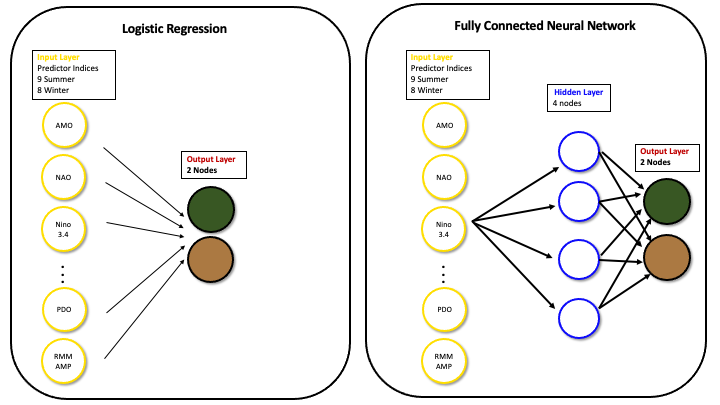
\includegraphics[width=35pc,angle=0]{Figure2.png}
  \caption{Schematic of Logistic Regression (left) and fully connected Neural Network (right) architectures.}\label{f2}
\end{figure}

\subsection{Convolutional Neural Network}
\label{sec:cnn}

Our results will show that predicting the sign of SEUS precipitation anomalies using perfect, \emph{a priori} defined predictors is both unskillful and unreliable (see Section \ref{sec:results}\ref{sec:resultsindex}). This indicates that these indices are not sufficient predictors for SEUS precipitation. Therefore, we also explore the use of relevant gridded fields as predictors. The idea is that the data may be able to tell us more specifically what features are most important for SEUS precipitation and provide new insights into understanding and detecting these mechanisms. For example, Mayer and Barnes (2021) use a fully connected NN to predict the sign of North Atlantic 500 hPa geopotential height on subseasonal timescales using vectorized fields of tropical outgoing longwave radiation (OLR). While using a single gridded input field works well in this case of predicting 500 hPa height, many mechanisms are hypothesized to contribute to SEUS precipitation predictability (see Section \ref{sec:intro}), requiring a large number of input fields. With so many predictors relative to the sample size, the problem becomes intractable since weights must be learned for every predictor connected to every node. A common approach in machine learning to address this is to use a convolutional neural network (CNN), which reduces the number of connections and weights to be learned in training the model by taking advantage of the spatial coherence of the data to learn low-level predictors \citep{krizhevsky_imagenet_2012}. CNNs are often used in image detection as a feature selector, then a fully connected NN is used for the final layer \citep[e.g.,][]{krizhevsky_imagenet_2012,zeiler_visualizing_2013}. In our implementation, the gridded fields associated with each of the hypothesized predictor fields are used as input to the CNN. Our CNN consists of three convolutional layers, each of which are followed by max pooling layers (Figure \ref{f3}). The third convolutional layer is followed by one fully connected layer and finally the output layer which is the same as the FC-NN output layer (Figure \ref{f3}). Further details of our CNN implementation are provided in Appendix C.

\begin{figure}[t]
  \noindent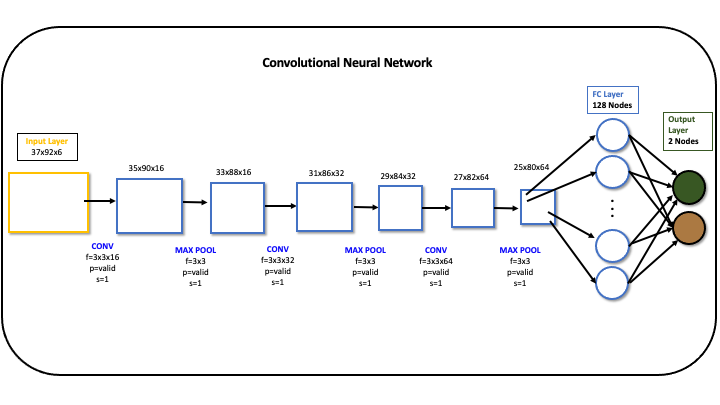
\includegraphics[width=35pc,angle=0]{Figure3.png}
  \caption{Schematic of Convolutional Neural Network architecture.}\label{f3}
\end{figure}

\subsection{Training, Validation, and Testing}
\label{sec:tvt}

In order to train and test the models, the data are split into training, validation, and testing sets.  The training data are used by the model to learn the weights associated with each predictor and node that can identify the known outcome.  Validation data are used to tune the parameters of the models such as number of layers and nodes, regularization, and learning rate in order to identify a model configuration that is both skillful and is not overfit to the training data.  The years 1979-2016 are used for training and validation, with 90\% ($N_{DJF}$=3087; $N_{JJA}$=3146) used for training and 10\% ($N_{DJF}$=383; $N_{JJA}$=350) for validation. Finally, testing data is held out until a model configuration is decided on and fully trained in order to ensure that the model generalizes to data it has not yet seen. The years 2017-2019 are used for testing ($N_{DJF}$=240; $N_{JJA}$=276).

\subsection{Layerwise Relevance Propagation}
\label{sec:lrp}

Following \citet{barnes_indicator_2020, toms_assessing_2021,toms_physically_2020,toms_testing_2021,mayer_subseasonal_2021}, we use layerwise relevance propagation (LRP) \citep{montavon_layer-wise_2019,bach_pixel-wise_2015} to understand what the NNs have learned about the relationships between the predictors and SEUS precipitation. Once a NN is trained, an input can be given to it to make a prediction. Using LRP, that prediction is then passed back through the trained network following specific rules to determine the relevance of each of the input predictors to the final prediction. The result is a “heat map” for each prediction that indicates a unitless relevance of each predictor to the output. Mayer and Barnes (2021) apply LRP to their NN to identify the OLR patterns most important for making successful and confident predictions of the sign of North Atlantic Z500. \citet{toms_physically_2020} use LRP to produce heat maps of El Ni\~no and La Ni\~na patterns correctly identified by a FC-NN using SST anomalies as predictors.  \citet{toms_testing_2021} use LRP to show how a FC-NN can accurately identify the known MJO spatial patterns when learning to detect the phase of the MJO based on clouds and circulation fields. We apply LRP to our FC-NN and CNN to identify sources of predictability for SEUS precipitation. Details of LRP and its implementation are provided in Appendix D.

\section{Results}
\label{sec:results}

\subsection{Skill and Reliability of Index-based Models}
\label{sec:resultsindex}

Despite the same architecture, the stochastic nature of the initialization and minimization procedure produces models with different weights, thus 100 models are trained and tested using the indices noted in Table \ref{t1}. The histogram of the accuracy (also called the hit rate) for the LR and FC-NN models is shown in Figure \ref{f4}. The hit rates demonstrate that the FC-NN and LR have similar skill. In both cases, the average skill is about 50\%, indicating that the models are no better than random chance in identifying the sign of SEUS precipitation anomalies using these indices as predictors. Even if overall skill is poor, perhaps there are forecasts of opportunity that can be identified based on the probabilities provided by the models, i.e., perhaps the forecasts with higher probabilities have a higher correct identification of the outcome \citep[e.g.,][]{mayer_subseasonal_2021}. This is quantified using reliability diagrams (Figure \ref{f5}) \citep{murphy_reliability_1977}. Reliability tells us how well the predicted probabilities of an event occurring corresponds to their observed frequencies. Neither the LR nor FC-NN can reliably identify the sign of SEUS precipitation even with perfect predictors. These results are underscored by the fact there is little consistency from forecast to forecast or across the models in the weights of the LR predictors or the predictors identified as most important using LRP with the FC-NN (not shown). This tells us that these predictors are not sufficient to accurately or reliably identify the sign of daily SEUS precipitation anomalies, even though the predictors are perfectly known. It also tells us that a complex model that can learn non-linear relationships does not produce better predictions than the logistic regression model when using the \emph{a priori} defined, index-based predictors.

\begin{figure}[t]
  \noindent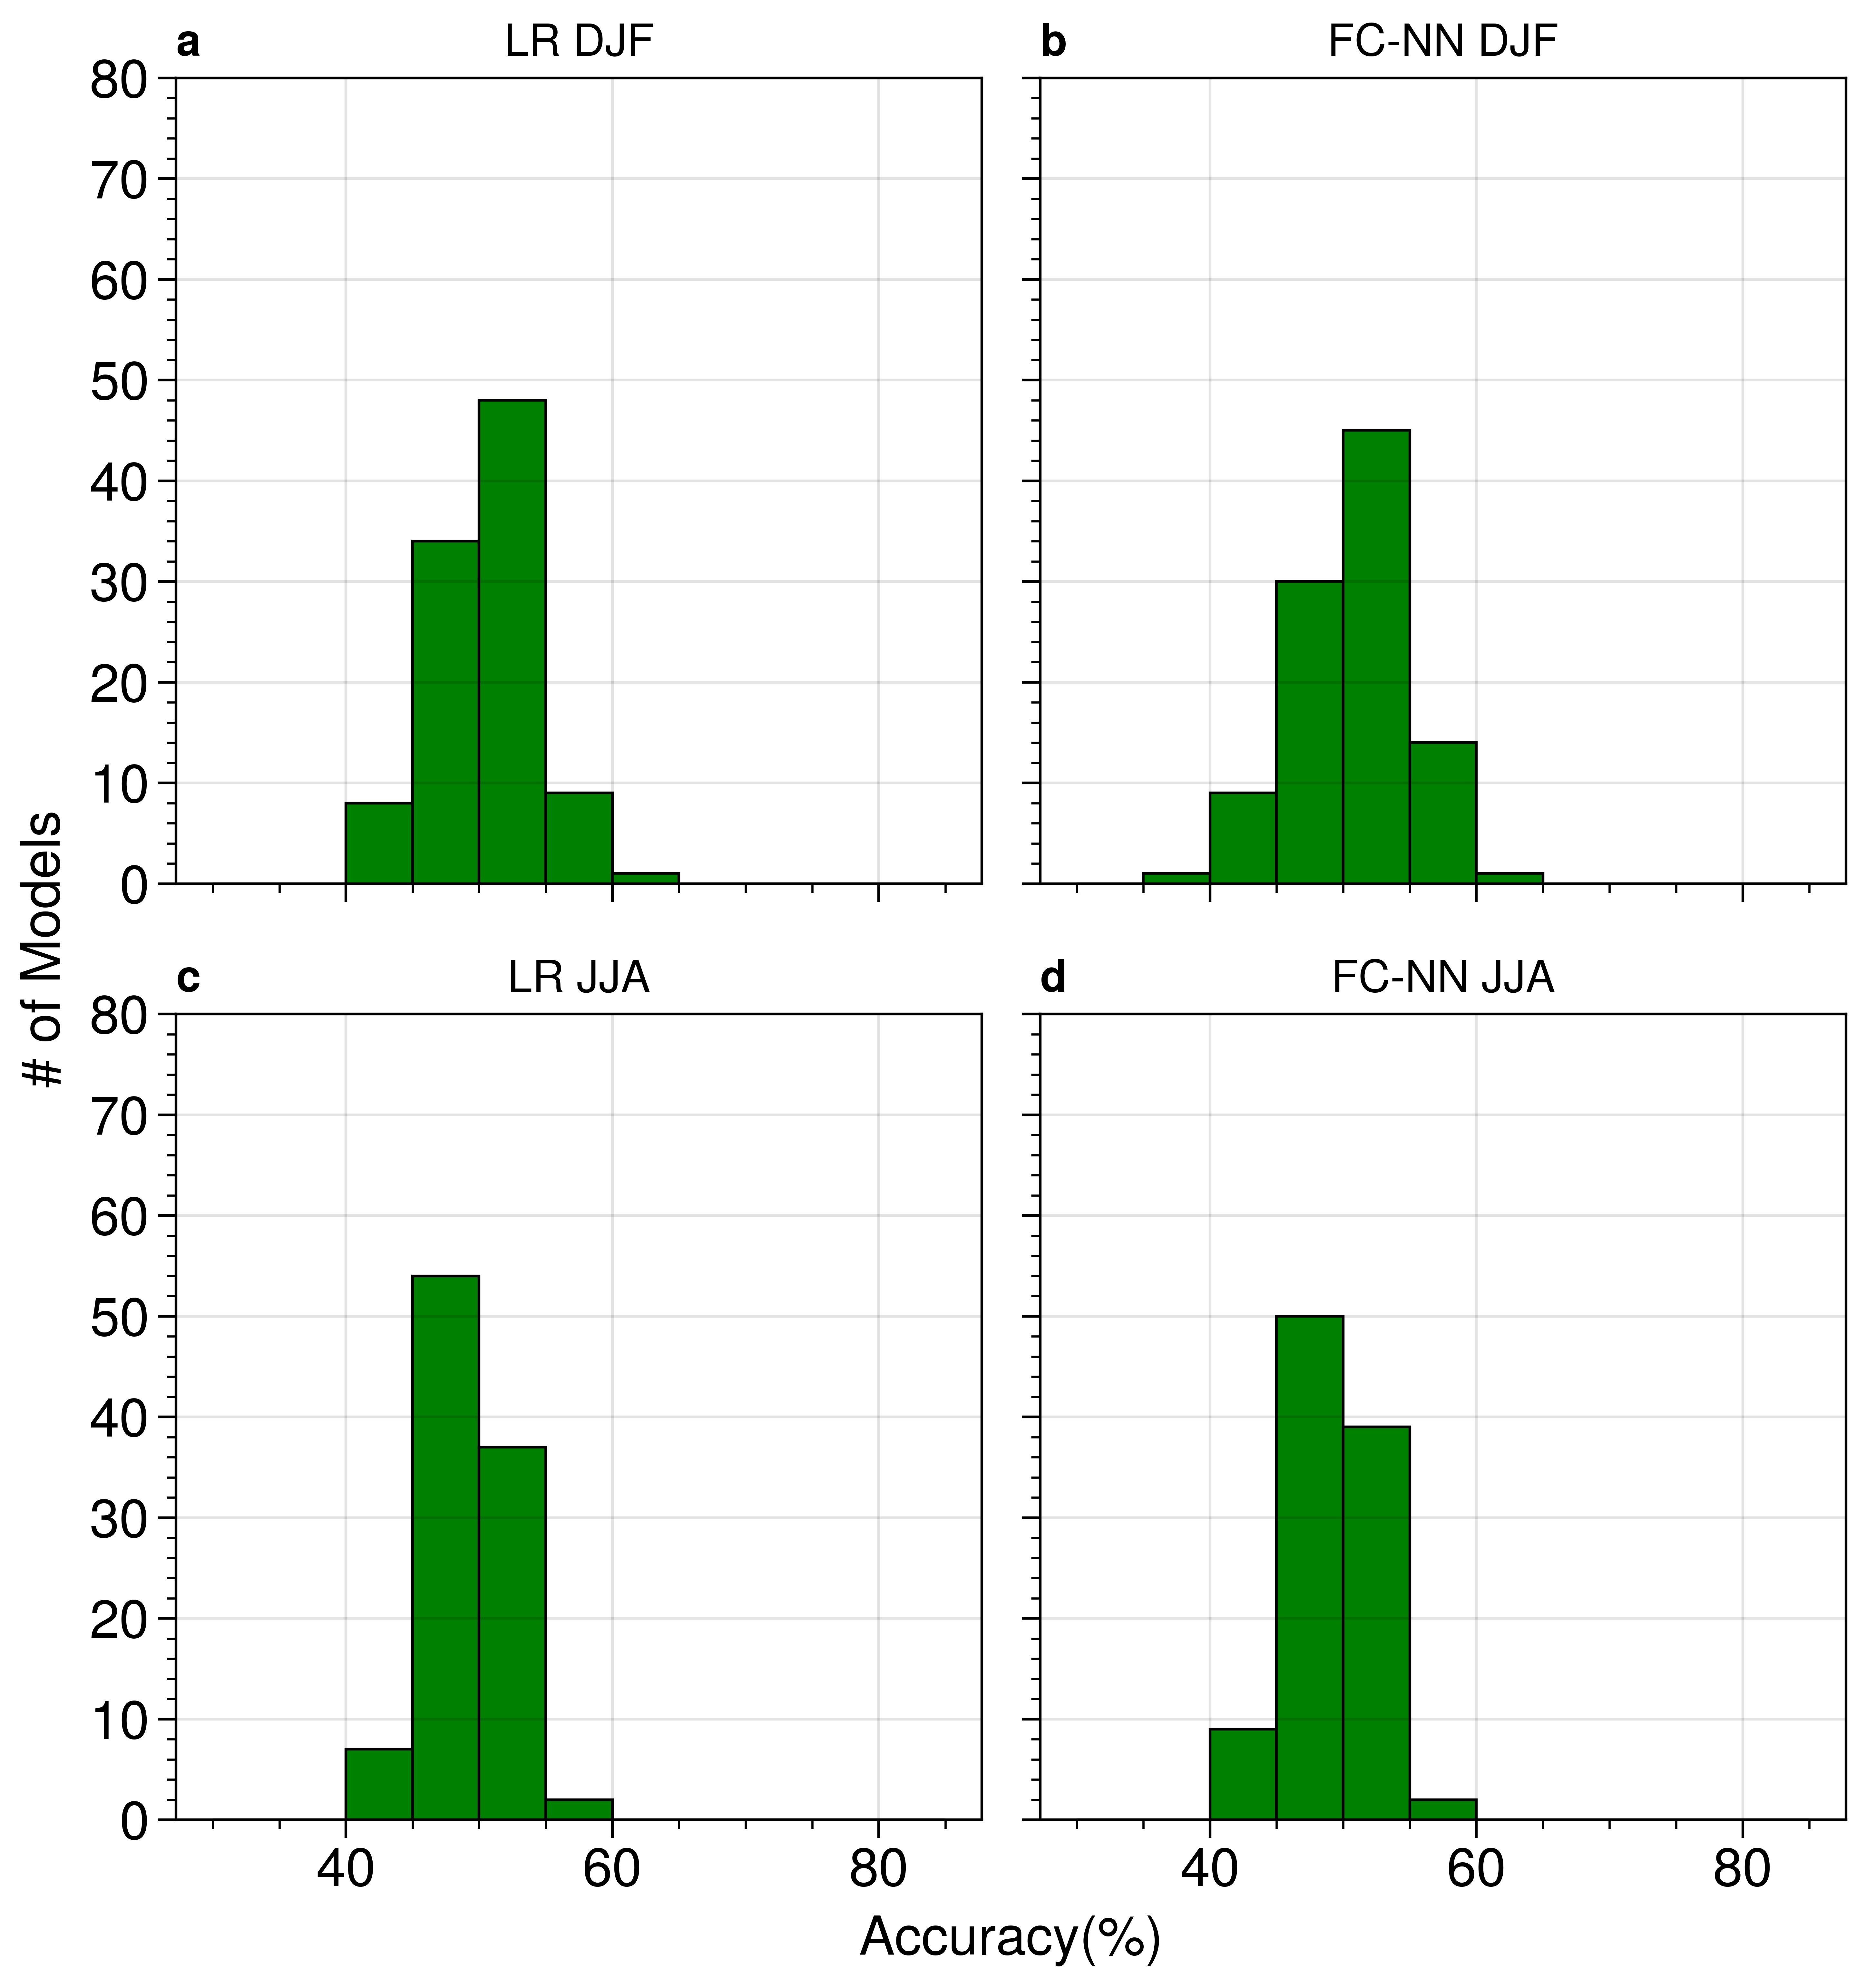
\includegraphics[width=20pc,angle=0]{Figure4.jpg}
  \caption{Histogram of test accuracy of 100 (a,c) Logistic Regression models and (b,d) fully connected Neural Network models (a,b) for winter and (c,d) summer.}\label{f4}
\end{figure}

\begin{figure}[t]
  \noindent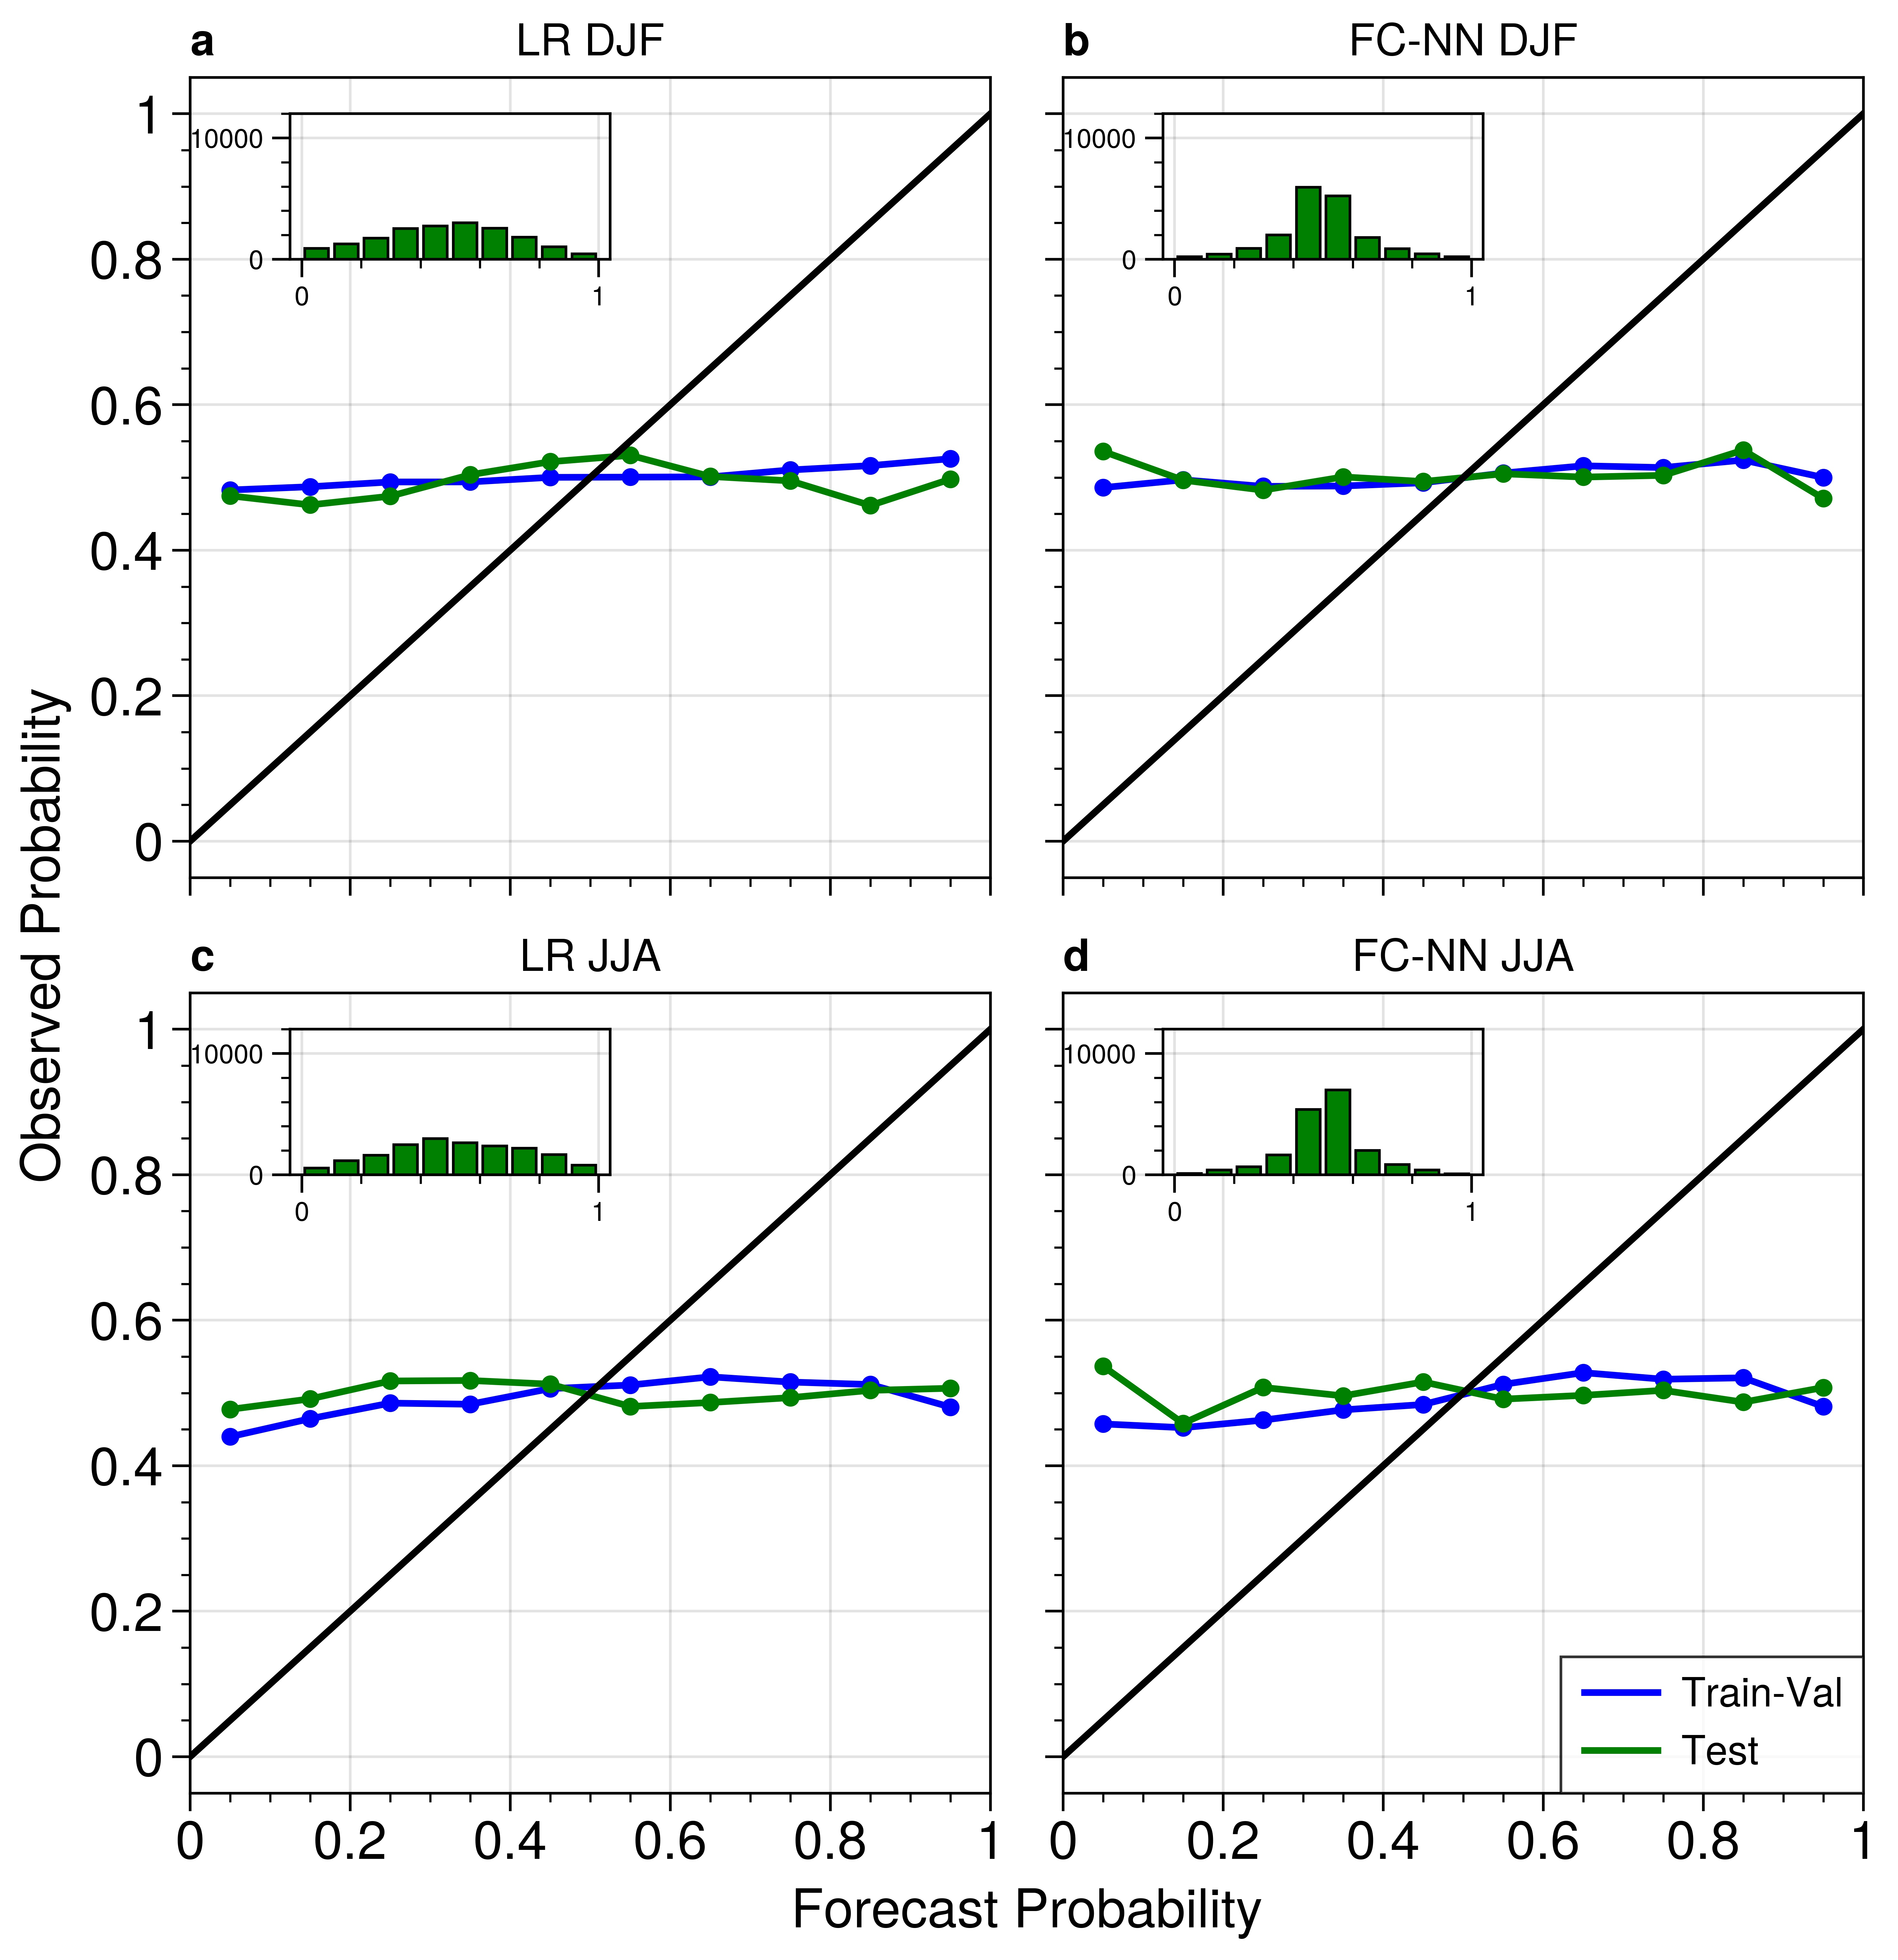
\includegraphics[width=30pc,angle=0]{Figure5.jpg}
  \caption{Reliability diagrams for positive precipitation anomalies using the index models for (a,c) LR and (b,d) FC-NN during (a,b) DJF and (c,d) JJA.  The x-axis indicates the predicted frequency and the y-axis indicates the observed frequency.  Test data are shown in green; training and validation data are shown in blue.  Insets show the number of forecasts in each frequency bin for test data.  Because there are two mutually exclusive categories, reliability is shown for the positive precipitation anomaly category.  Negative precipitation reliability is 1-positive precipitation reliability.}\label{f5}
\end{figure}

\subsection{Skill and Reliability of Grid-based Models}
\label{sec:resultsgrid}

Next we test the skill and reliability of the models using gridded ERA-Interim fields of anomalous global SST, U200, U850, Z500, Z850, and tropical OLR as predictors which allows the CNN to identify the predictors from the data rather than defining them \emph{a priori}. Similar to the previous section, 100 CNNs are trained. For winter and summer, the CNN is more accurate (Figure \ref{f6}) and reliable (Figure \ref{f7}) than the index based models. This means that for these models, the probabilities can be used as a reliable measure of forecast confidence for any given forecast. Since the CNN forecasts are accurate and reliable, we will use them to explore and understand sources of predictability based on the forecast confidence.

\begin{figure}[t]
  \noindent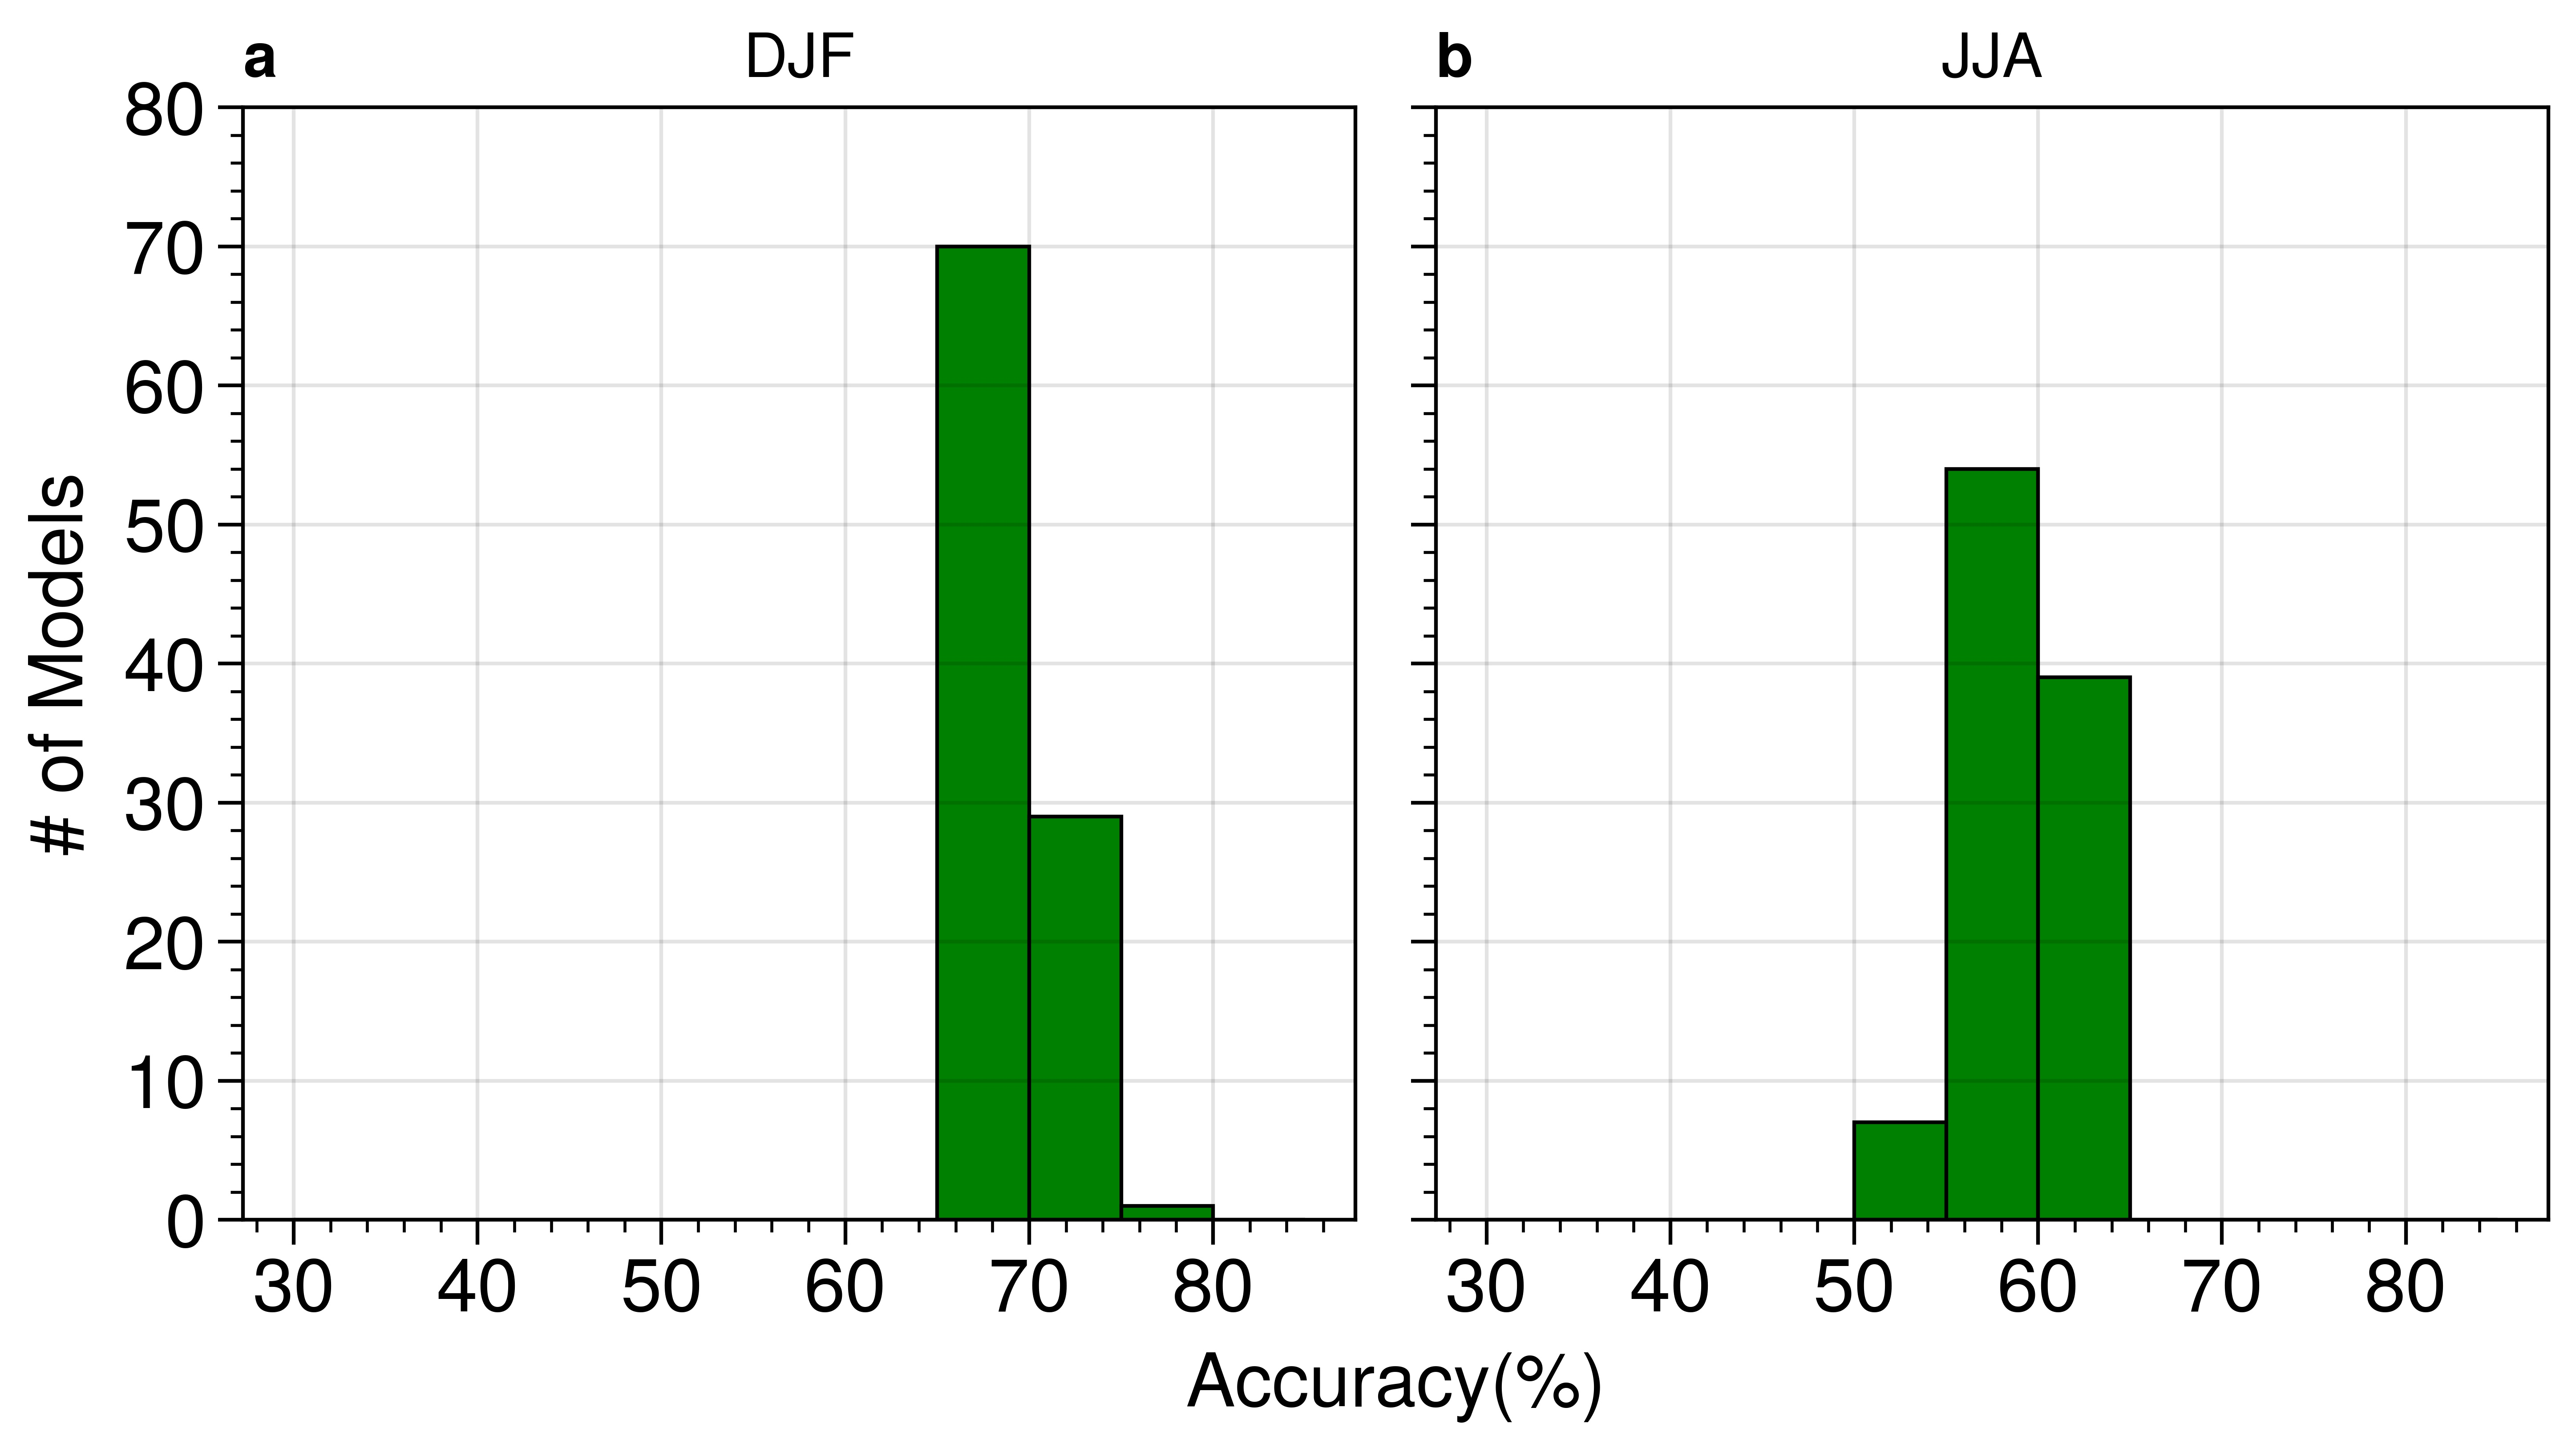
\includegraphics[width=20pc,angle=0]{Figure6.jpg}
  \caption{Histogram of test accuracy from 100 CNNs for (a) DJF and (b) JJA.}\label{f6}
\end{figure}


\begin{figure}[t]
  \noindent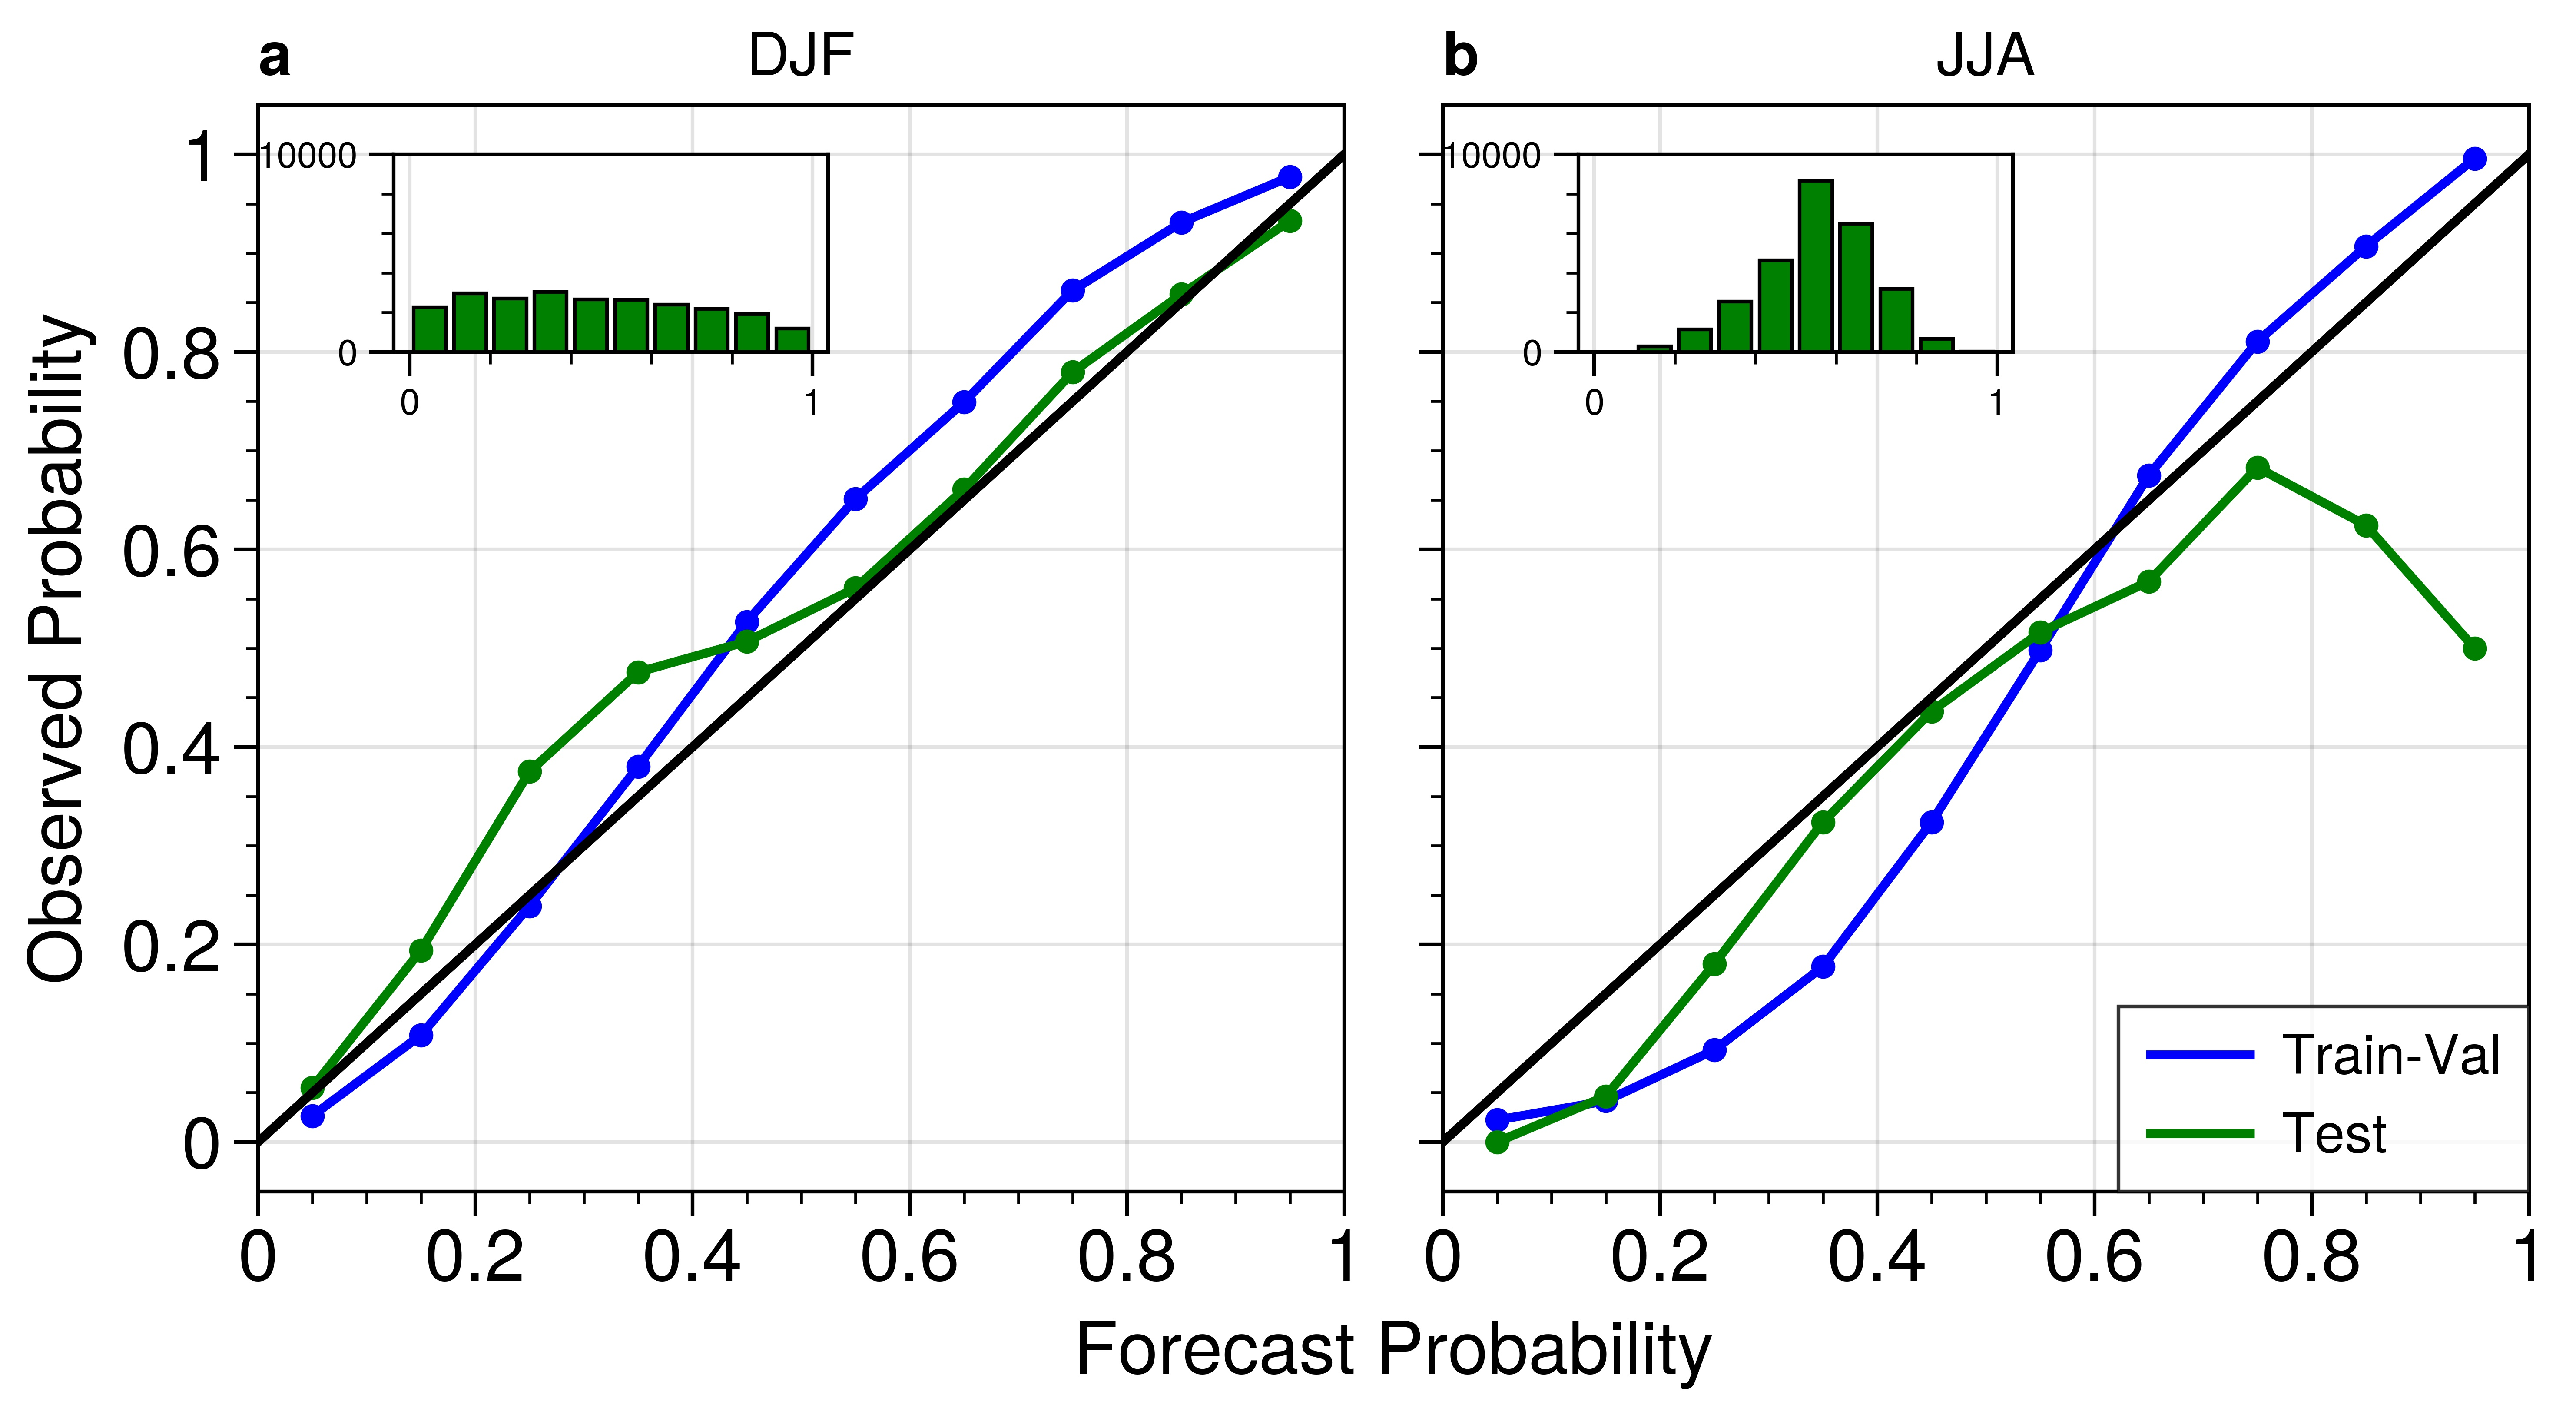
\includegraphics[width=35pc,angle=00]{Figure7.jpg}
  \caption{Reliability diagrams for positive precipitation anomalies using the CNN models for (a) DJF and (b) JJA.  The x-axis indicates the predicted frequency and the y-axis indicates the observed frequency. Test data are shown in blue; training and validation data are shown in green. Insets show the number of forecasts in each frequency bin for test data.  Because there are two mutually exclusive categories, reliability is only shown for the positive precipitation anomaly category.  Negative precipitation reliability is 1-positive precipitation reliability. Less reliable test data for high probability JJA forecasts is due to the small number of samples in those categories.}\label{f7}
\end{figure}

\subsection{Sources of Predictability for Positive Anomalies of SEUS Precipitation}
\label{sec:resultspos}

In order to explore the sources of predictability for SEUS Rainfall, we use layerwise relevance propagation (LRP) to identify the predictors (i.e., gridpoints) most relevant to the prediction of confident (>=80\% probability) forecasts of positive and negative precipitation anomalies. Composites are also used to relate unitless LRP relevance to physical quantities. The relevance and composites for confident, correct forecasts of above-normal SEUS precipitation are shown in Figures \ref{f8} and \ref{f9}. Relevance values are normalized by the relevance of all other predictors (i.e., gridpoints and variables) such that the variable and gridpoint with the highest value in any given forecast is one. 

The anomalous low 850 hPa gepotential height over the Gulf of Mexico and associated 850 hPa zonal wind anomalies have the strongest relevance during winter (Fig \ref{f9}a,c).  This circulation brings moisture from the Gulf of Mexico into the SEUS and is  coincident with El Ni\~{n}o-related SST and OLR anomalies in the tropical Pacific (Figure \ref{f8}e). The SST and OLR anomalies show no relevance compared to the circulation fields.  This is not surprising given our perfect predictor experiment design, since the large-scale, remote impact of SST and OLR on precipitation occurs through changes in circulation \citep[e.g.,][]{ropelewski_north_1986}.  The winter relevance and composites show results consistent with well-known winter teleconnection patterns associated with ENSO \citep[e.g.,][]{ropelewski_north_1986}. This provides further evidence that the CNN can learn and LRP can identify physical relationships. 

During the summer, the strongest relevance is associated with positive 850hPa height anomalies and corresponding 850 hPa winds.  This circulation is consistent with a northwest shift of the NASH and dry conditions over the SEUS (Figure \ref{f9}c). There is also relevance about 30\% of the maximum relevance associated with SST anomalies in the NASH region and in the north Atlantic, consistent with the AMO-NASH hypothesis for SEUS precipitation (Figure \ref{f8}c).

\begin{figure}[t]
  \noindent\includegraphics[width=30pc,angle=0]{Figure8.jpg}
  \caption{Composite anomalies of (a,c) SST ($^\circ$C) and (b,d) OLR ($Wm^{-2}$) (contours), normalized relevance (gray-scale shading) for confident (>=80\% probability) and correct forecasts of positive precipitation anomalies over training, validation, and test data for (a,b) DJF and (c,d) JJA}\label{f8}
\end{figure}

\begin{figure}[t]
  \noindent\includegraphics[width=30pc,angle=0]{Figure9.jpg}
  \caption{Composite anomalies of (a,c) Z500 (m) (contours) and 200 hPa winds ($ms^{-1}$) (vectors) and (b,d) Z850 (m) (contours) and 850 hPa winds ($ms^{-1}$) (vectors) and normalized relevance of 850hPa and 200hPa geopotential height (gray-scale shading) and zonal winds (green-scale shading) for confident (>=80\% probability) and correct forecasts of positive precipitation anomalies over training, validation, and test data for (a,b) DJF and (c,d) JJA}\label{f9}
\end{figure}

\subsection{Sources of Predictability for Negative Anomalies of SEUS Precipitation}
\label{sec:resultsneg}

Confident, correct forecasts for negative precipitation anomalies in the SEUS are shown in Figures \ref{f10} and \ref{f11}. The locations and corresponding composites are similar to the positive precipitation forecasts but with opposite sign. The 850 hPa zonal winds and geopotential heights enhances flow of continental air over the SEUS.  These conditions occur during weak La Ni\~{n}a SST anomalies and near zero tropical OLR anomalies (Figure \ref{f10}). The relevant 850hPa heights and winds during summer are consistent with a southwestward shift of the NASH. (Figure \ref{f10}). Corresponding summer SST anomalies are cold in the central tropical Pacific, and strong in the subtropical and mid-latitude Pacific, but have weak relevance compared to the circulation fields. 

\begin{figure}[t]
  \noindent\includegraphics[width=30pc,angle=0]{Figure10.jpg}
  \caption{Composite anomalies of (a,c) SST ($^\circ$C) and (b,d) OLR ($Wm^{-2}$) (contours), normalized relevance (gray-scale shading) for confident (>=80\% probability) and correct forecasts of negative precipitation anomalies over training, validation, and test data for (a,b) DJF and (c,d) JJA}\label{f10}
\end{figure}

\begin{figure}[t]
  \noindent\includegraphics[width=30pc,angle=0]{Figure11.jpg}
  \caption{Composite anomalies of (a,c) Z500 (m) (contours) and U200 ($ms^{-1}$) (vectors) and (b,d) Z850 (m) (contours) and U850 ($ms^{-1}$) (vectors) and normalized relevance (gray-scale shading) for confident (>=80\% probability) and correct forecasts of negative precipitation anomalies over training, validation, and test data for (a,b) DJF and (c,d) JJA}\label{f11}
\end{figure}

\subsection{Timescales of Predictability}
\label{sec:restimescale}

In order to further understand these composite patterns as sources of predictability, we investigate their timescales.  The composite patterns are treated as a basis set and a corresponding timeseries associated with each pattern is calculated by projecting the original anomalies for each variable onto its composite pattern for confident, successful forecasts of positive and negative precipitation anomalies (i.e., the patterns shown in Figures \ref{f8},\ref{f9},\ref{f10}, and \ref{f11}).  The projections are calculated separately for DJF and JJA. To quantify the dominant timescales for each of these timeseries, power spectra are estimated using the \citet{welch_use_1967} method in scipy.signal \citep{virtanen_scipy_2020} which calculates the power spectra for overlapping segments of data and then averages the spectra for each segment to produce a smooth periodogram.  Corresponding red noise spectra are also calculated based on the estimated de-correlation time ($T_e$) of the timeseries of each composite for each variable (Table \ref{t2}). There is no significant power above a red noise spectra for any of the variables in winter or summer (not shown).  This indicates that the timescales of predictability for these patterns are primarily associated with their persistence.

\begin{table}[t]
\caption{Table of De-correlation Times.  Plus sign (+) indicates timeseries from positive precipitation anomalies.  Minus sign (-) indicates timeseries from negative precipitation anomalies}\label{t2}
\begin{center}
\begin{tabular}{ccc}
\hline\hline
$Variable$ & $T_e DJF (Days)$ & $T_e JJA (Days) $ \\
\hline
SST & +824/-341 & +422/-208 \\
OLR & +16/-6 & +4/-4 \\
Z500 & +7/-6 & +8/-8 \\
Z850 & +7/-5 & +7/-7\\
U200 & +6/-5 & +5/-5 \\
U850 & +4/-4 & +4/-3 \\
\hline
\end{tabular}
\end{center}
\end{table}

\section{Conclusion and Discussion}
\label{sec:conclusion}

We investigate sources of predictability for daily precipitation in the SEUS using perfect predictor experiments with machine learning models.  Many studies have provided evidence of large-scale climate phenomena that impact SEUS precipitation; this study explores how well we can predict the sign of daily SEUS precipitation anomalies if these large-scale climate predictors are known perfectly, and which of these predictors are most important.  A logistic regression and fully connected neural network trained using indices representing the large-scale climate phenomena as predictors are neither skillful nor reliable.  This tells us that these climate indicates are not sufficient to predict the sign of daily precipitation anomalies, even if they are known perfectly.  While a FC-NN is capable of representing non-linear and linear relationships, the fact that it has similar skill (~50\% accuracy) and lack of reliability as the logistic regression model indicates that the inability to predict the sign of SEUS precipitation anomalies is because the indices are not good predictors. Based on this, we can conclude that using indices of large-scale climate phenomena is insufficient to skillfully or reliably predict the sign of daily precipitation anomalies in the SEUS.

The finding that neither the logistic regression nor the fully connected neural network can predict daily precipitation is not an unexpected outcome. While subseasonal and seasonal climate patterns are known to influence the statistics of regional precipitation averaged over weeks or months \citep[e.g.,][]{ropelewski_north_1986,ropelewski_global_1987,higgins_dominant_2000}, due to the high internal variability of precipitation, we would be surprised if we could predict even the sign of a single-day precipitation anomaly given only several climate indexes. This specific analysis was undertaken to provide a baseline for the prediction of daily precipitation using full atmospheric fields in a CNN, which is found to be much more successful. However, future work will test this methodology in the context of higher-predictability fields, such as the frequency of precipitation during a subseasonal period, the number of dry or wet spells, or subseasonal extreme precipitation. We would also be curious to see how the combination of several climate indexes in an ML context performs with the prediction of daily temperature or heat waves.  

Global gridded fields as predictors in a CNN produce more accurate predictions (~70\% for winter; ~60\% for summer) and the predictions in both winter and summer are reliable. This allows us to use the probability for each forecast category as a forecast confidence to identify forecasts of opportunity, following \cite{mayer_subseasonal_2021}.  We use the forecast confidence and and layerwise relevance propagation to identify the most relevant predictors for confident (>=80\%) and correct forecasts.  For both positive and negative precipitation anomalies, the most relevant predictors are identified as the local zonal wind and geopotential height anomalies at 850hPa.  These circulation anomalies cannot be clearly identified as related to any well-known extratropical pattern of variability, although some regional elements are similar.  Additionally, even with perfect predictors, the sign of SEUS precipitation anomalies are not perfectly predicted.  To correctly predict even the sign of daily precipitation anomalies in the SEUS, skillful predictions of the local circulation are required.  Composites of corresponding SST and OLR anomalies point to a relationship between the circulation and well-known large-scale climate phenomena such as ENSO during winter and the AMO-NASH during summer.  However, just using indices of these phenomena did not lead to skillful prediction.  This is because there is large uncertainty in the SEUS circulation anomalies associated with large-scale climate variability \citep[e.g.,][]{deser_how_2018}.  We also find that the timescales of these predictors are associated with their persistence.

These perfect predictor experiments are idealized--the values of these predictors would not be known at forecast time in a true forecasting situation.  A more realistic prediction would be obtained by using either predicted variables as input to our ML models or observed data at some forecast lead time.  We argue that these experiments show an upper limit to predicting the sign of precipitation anomalies in the SEUS based on available training data.  Errors in the predictors will produce even less accurate predictions.  Future work will explore how errors in the predictor fields lead to errors in precipitation at various lead-times.  It is also important to note that daily precipitation is an extremely difficult prediction to make and many aspects of it may not be predictable using these predictors (e.g., mesoscale and synoptic variability).  

%%%%%%%%%%%%%%%%%%%%%%%%%%%%%%%%%%%%%%%%%%%%%%%%%%%%%%%%%%%%%%%%%%%%%
% TABLES---INSERT NEAR IN-TEXT DISCUSSION
%%%%%%%%%%%%%%%%%%%%%%%%%%%%%%%%%%%%%%%%%%%%%%%%%%%%%%%%%%%%%%%%%%%%%
%%  Enter tables near where they are discussed within the document. 
%%  Please place tables before/after paragraphs, not within a paragraph.
%%
%
%\begin{table}[t]
%\caption{This is a sample table caption and table layout.  Enter as many tables as
%  necessary at the end of your manuscript. Table from Lorenz (1963).}\label{t1}
%\begin{center}
%\begin{tabular}{ccccrrcrc}
%\hline\hline
%$N$ & $X$ & $Y$ & $Z$\\
%\hline
% 0000 & 0000 & 0010 & 0000 \\
% 0005 & 0004 & 0012 & 0000 \\
% 0010 & 0009 & 0020 & 0000 \\
% 0015 & 0016 & 0036 & 0002 \\
% 0020 & 0030 & 0066 & 0007 \\
% 0025 & 0054 & 0115 & 0024 \\
%\hline
%\end{tabular}
%\end{center}
%\end{table}

%%%%%%%%%%%%%%%%%%%%%%%%%%%%%%%%%%%%%%%%%%%%%%%%%%%%%%%%%%%%%%%%%%%%%
% FIGURES---INSERT NEAR IN-TEXT DISCUSSION
%%%%%%%%%%%%%%%%%%%%%%%%%%%%%%%%%%%%%%%%%%%%%%%%%%%%%%%%%%%%%%%%%%%%%
%%  Enter figures near where they are discussed within the document.
%%  Please place figures before/after paragraphs, not within a paragraph.
% %
%
%\begin{figure}[t]
%  \noindent\includegraphics[width=19pc,angle=0]{figure01.pdf}\\
%  \caption{Enter the caption for your figure here.  Repeat as
%  necessary for each of your figures. Figure from \protect\cite{Knutti2008}.}\label{f1}
%\end{figure}

\clearpage
%%%%%%%%%%%%%%%%%%%%%%%%%%%%%%%%%%%%%%%%%%%%%%%%%%%%%%%%%%%%%%%%%%%%%
% ACKNOWLEDGMENTS
%%%%%%%%%%%%%%%%%%%%%%%%%%%%%%%%%%%%%%%%%%%%%%%%%%%%%%%%%%%%%%%%%%%%%
\acknowledgments
K.P. thanks K. Huang for assistance downloading data.  B.K. acknowledges the support from NOAA (NA20OAR4320472, NA18OAR4310293), NSF (OCE1419569, OCE1559151), and DOE (DE-SC0019433).  
%  Keep acknowledgments (note correct spelling: no ``e'' between the ``g'' and
% ``m'') as brief as possible. In general, acknowledge only direct help in
%  writing or research. Financial support (e.g., grant numbers) for the work done, 
%  for an author, or for the laboratory where the work was performed must be 
%  acknowledged here rather than as footnotes to the title or to an author's name.
%  Contribution numbers (if the work has been published by the author's institution 
%  or organization) should be placed in the acknowledgments rather than as 
%  footnotes to the title or to an author's name.

%%%%%%%%%%%%%%%%%%%%%%%%%%%%%%%%%%%%%%%%%%%%%%%%%%%%%%%%%%%%%%%%%%%%%
% DATA AVAILABILITY STATEMENT
%%%%%%%%%%%%%%%%%%%%%%%%%%%%%%%%%%%%%%%%%%%%%%%%%%%%%%%%%%%%%%%%%%%%%
% 
%
\datastatement
%  The data availability statement is where authors should describe how the data underlying 
%  the findings within the article can be accessed and reused. Authors should attempt to 
%  provide unrestricted access to all data and materials underlying reported findings. 
%  If data access is restricted, authors must mention this in the statement. See
%  {http://www.ametsoc.org/PubsDataPolicy} for more info.
Monthly climate indices for the AMO, NAO, and Ni\~{n}o3.4 are publicly available from NOAA/ESRL/PSL at https://psl.noaa.gov/data/climateindices/list/.
The real-time multivariate MJO indices are publicly available from http://www.bom.gov.au/climate/mjo/.
ERA-Interim data is available from https://www.ecmwf.int/en/forecasts/datasets/reanalysis-datasets/era-interim. Codes for this project are available on Github (https://github.com/kpegion/ml-precip).  Pacific North America weather regimes, MLSO, and NASH can be calculated from ERA-Interim using the codes provided. The codes used to produce the LR, FC-NN, and CNN models are also provided. LRP is applied using the investigate toolkit and is available on Github https://github.com/albermax/innvestigate
%%%%%%%%%%%%%%%%%%%%%%%%%%%%%%%%%%%%%%%%%%%%%%%%%%%%%%%%%%%%%%%%%%%%%
% APPENDIXES
%%%%%%%%%%%%%%%%%%%%%%%%%%%%%%%%%%%%%%%%%%%%%%%%%%%%%%%%%%%%%%%%%%%%%
%
%% If only one appendix, use

%\appendix

%% If more than one appendix, use \appendix[<letter>], e.g.,

%\appendix[A] 

%% Appendix title is necessary! For appendix title:

%\appendixtitle{Title of Appendix}

%%% Appendix section numbering (note, skip \section and begin with \subsection)
%
% \subsection{First primary heading}

% \subsubsection{First secondary heading}

% \paragraph{First tertiary heading}
\appendix[A] 
\appendixtitle{Logistic Regression Implementation}
\label{appendix:A}
Logistic regression is used as a baseline, simplest possible model for our two-class problem of predicting yes or no for positive precipitation anomalies and yes or no for negative precipitation anomalies. It can be viewed as a neural network with no hidden nodes. It contains an input layer of predictors ($x$) and an output layer that predicts the probability of a given output class (e.g. positive or negative anomalies) based on an input $x_i$ as follows:

\begin{equation}
\label{eq:1}
\hat{y}=\sigma(z_i) = P( Pos, Neg | x_i)
\end{equation} where 

\begin{equation}
\label{eq:2}
z_i=w^Tx_{i}+b
\end{equation} and 

\begin{equation}
\label{eq:3}
\sigma(z)=\frac{1}{1+e^{-z}}
\end{equation}

The predictors ${x}$ for our problem are the indices in Table \ref{t1}. The weights ($w$) and biases ($b$) associated with each predictor are determined by minimizing the cross-entropy loss function over all training samples ($m$): 

\begin{equation}
\label{eq:4}
J(w,b)=-\sum_{i=1}^{m}{y_{i}log(\hat{y}_{i})},
\end{equation}

Minimization of the loss function is determined by numerically estimating its derivative, $\frac{dJ(w,b)}{dw}$ through backpropagation.  For a given training sample, once the output is determined, the partial derivatives of the loss function due to each node are determined by going backwards through the network.  These partial derivatives are combined to determine the total errors for a given prediction in a chain-rule like fashion.   

Finally, the softmax function is applied to the output layer to convert the probabilities to a categorical outcome (i.e., yes/no) for each of the two categories. 

\begin{equation}
\label{eq:5}
\hat{y}_{i}=\frac{e^{z_i}}{\sum{e^{z_i}}}
\end{equation}

The target values of $y_i$ are set to ones and zeros for each category using one-hot encoding. The median of the precipitation anomalies is removed prior to the encoding to ensure balanced target classes. 

To train our logistic regression model, we use mini-batch gradient descent with a batch size of 25 and 250 epochs.  A learning rate of $10^{-5}$ is used with the Adam optimization method \citep{kingma_adam_2017}.

\appendix[B] 
\appendixtitle{Fully Connected Neural Network Implementation}
\label{BFCNN}
The weights ($w$) and biases ($b$) of the fully connected neural network are trained using the same procedure as the LR model.  However, the FC-NN has hidden layers and nodes that allow it to learn more complex, relationships between the predictors and target.  The value of a given node in a specific layer $a(z_j$) of the FC-NN is determined by minimizing the cross-entropy loss function (Equation \ref{eq:4}), then applying the nonlinear Rectified Linear unit (ReLU) activation function, 

\begin{equation}
\label{eq:6}
a(z_j)=max(0,z_j)
\end{equation}

This is repeated for each layer and node in the FC-NN until the output layer where the softmax function is used to identify the predicted category (Equation \ref{eq:5}).  

For the FC-NN minimization, the weights of the nodes must be initialized to small random non-zero values to start the gradient descent.  The He Normal initialization \citep{he_deep_2016} is used to initialize the weights. The same learning rate and Adam optimization were used to train our FC-NN as was used for the LR.  A range of hidden layers, nodes, and regularization were tested.  The selected model produced the most similar accuracy between the train and validation data and the most reliable predictions in training and validation.  This model is relatively simple with only one hidden layer containing four nodes and no regularization.  More complex models led to overfitting even with regularization.
                      
\appendix[C] 
\appendixtitle{Convolutional Neural Network Implementation}
\label{CCNN}
A CNN involves applying convolutional filters to the input data for each node to take advantage of spatial coherence of the data to learn the predictors and reduce the number of weights and biases that must be learned relative to a FC-NN \citep{krizhevsky_imagenet_2017}. The convolution ($C$) of a matrix $A$ of size $n_h x n_w x n_c$ with a filter $F$ of size $fxfxn_c$ is as follows:

\begin{equation}
\label{eq:7}
C_{ij}=(A*F)_{ij}=\sum_{p=0}^{f-1}\sum_{q=0}^{f-1}\sum_{r=0}^{n_c-1}A_{i+p,j+q,r}*F_{pqr}
\end{equation}
The convolution can be applied to the matrix $A$ with multiple filters. Our CNN architecture uses 16, 32, and 64 filters respectively.  Each filter is size 3x3 with valid padding and a stride of 1. 

The value of a node ($i$) in a given convolutional layer ($l$) of a CNN is calculated as:

\begin{equation}
\label{eq:8}
Z_i^{l}=A*F_i+b_i
\end{equation}

Then the non-linear ReLu activation function is applied to $Z_i^{l}$ (Equation \ref{eq:5}).

Following each convolutional layer, a max pooling layer is applied with valid padding to select the predictor (e.g. gridpoint) that has the maximum activation over each 3x3 grid. Ridge regularization (L2) is applied in the first and second convolutional layers with a value of $\lambda=20$ and $\lambda=10$ respectively.  Finally after the third convolutional and maxpooling layer, the outputs are flattened and treated as input for a FC-NN with 128 nodes. No regularization is applied to the third convolutional layer or FC-NN layer.  The softmax function (Equation \ref{eq:5}) is then applied to identify the yes/no outcome for the two classes of negative and positive precipitation anomalies. 

The input features to our CNN are the coarse grained, global gridded data fields of SST, Z500, Z850, U850, U200, and tropical OLR (zeroed out poleward of 30$^\circ$). In order to maintain the periodicity of the predictors in longitude during convolution, the input predictor fields are padded with a periodic halo of $p=10$ points in the longitude direction.  For our input data, $n_h=37, n_w=72+2p, n_c=6$. To train the CNN, we use a batch size of 25 and 100 epochs with early stopping after the validation loss increases for more than 2 epochs in a row.  Training generally takes between 55 and 65 epochs.  A learning rate of $3x10^{-5}$ and Adam optimization method are used.  The regularization parameters, number of layers and nodes were determined through training and validation.  The selected model produced the most similar accuracy between the train and validation data and the most reliable predictions in training and validation. The contingency table (also called confusion matrix) for an example CNN model is shown in Figure \ref{fC1}. It shows that the skill difference between winter and summer is primarily associated with false negatives, meaning that the model too often predicts precipitation when it does not occur.

 \begin{figure}[t]
  \noindent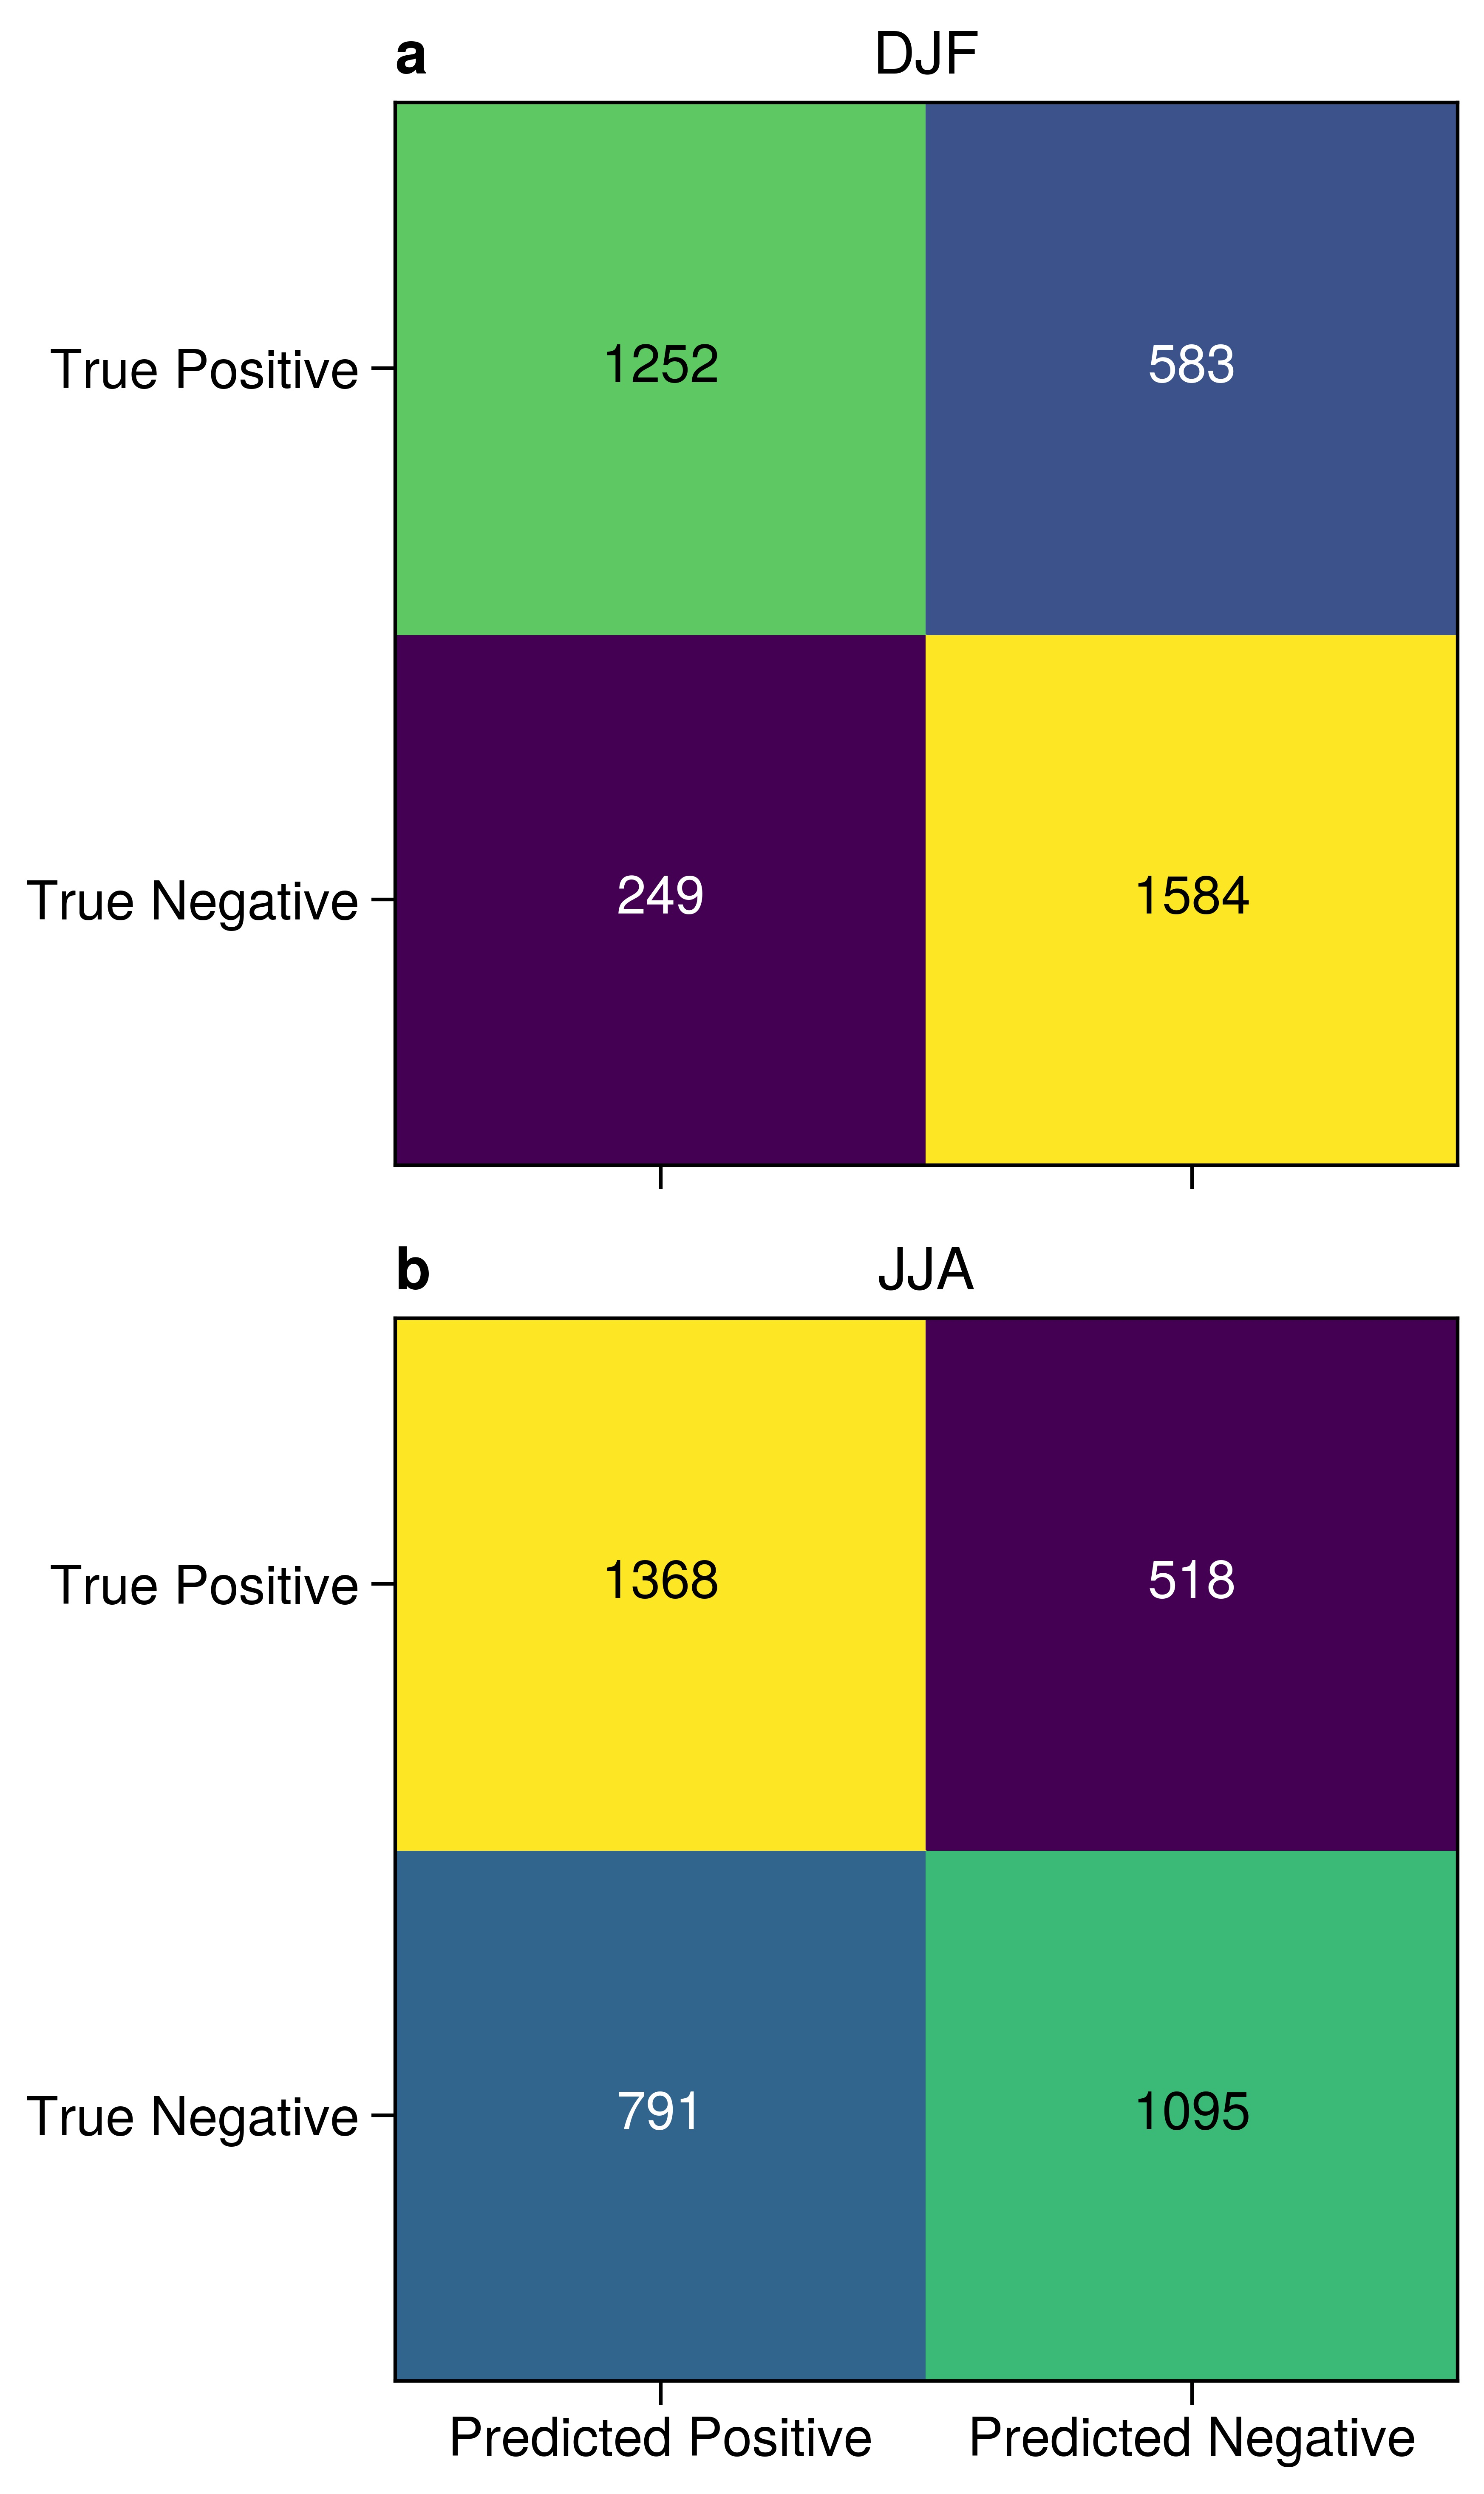
\includegraphics[width=30pc,angle=0]{FigureC1.jpg}
  \caption{Contingency tables for a selected model from the DJF and JJA Convolutional Neural Networks}\label{fC1}
\end{figure}

\appendix[D] 
\appendixtitle{Layerwise Relevance Propagation Implementation}
\label{DLRP}
LRP is applied to the FC-NN and CNN to identify which input predictors are most important to the predicted output of the model for any given prediction.  We utilize the innvestigate toolkit \citep{alber_innvestigate} to apply LRP.  For any given input to the model with output y,  LRP goes back through the model and determines for each node what input was most relevant to the output until the input nodes are reached.  We utilize the LRP-$\alpha\beta$ rule which can determine a relevance for inputs that contribute both positively ($\alpha$) and negatively ($\beta$) to the model output y.  We use $\alpha=1$ and $\beta=0$ to select only inputs that contribute positively to the predicted outcome of the model. The relevance $R$ of a given input, $j$,  to an output $k$ for this rule is given by the weighted value of the pre-softmax activation of a positively contributing node divided by the weighted sum of all previous pre-softmax nodes then multiplied by the total relevance of the previous node (Equation \ref{eq:9}).  The denomenator ensures that total relevance is a conserved quantity: 

\begin{equation}
\label{eq:9}
R_j=\sum_{j}{\frac{(a_{j}w_{jk})^+}{\sum_{0,j}{(a_{j}w_{jk})^+}}}R_{k}
\end{equation}

Once we determine the relevance of each predictor for all forecasts in the training and testing set, we then look for consistency between the predictors identified as most relevant to identify sources of predictability. 

\appendix[E]
\appendixtitle{Software and Code Implementation}
\label{ECODE}
The models used in this paper are written using Keras and Tensorflow. LRP is applied using the innvestigate package \citep{alber_innvestigate}.  Data preprocessing uses xarray \citep{hoyer_xarray_2017,hoyer_xarray_2021}, numpy \citep{harris_array_2020}, scipy \citep{virtanen_scipy_2020}, and scikit-learn \citep{pedregosa_scikit-learn_2011}.  Plotting is done using matplotlilb \citep{hunter_matplotlib_2007} and proplot \citep{davis_proplot_2021}. Reliability is calculated using xskillscore (https://xskillscore.readthedocs.io/en/stable/).  The codes used in this paper are publicly available in Github (https://github.com/kpegion/ml-precip).  

%%%%%%%%%%%%%%%%%%%%%%%%%%%%%%%%%%%%%%%%%%%%%%%%%%%%%%%%%%%%%%%%%%%%%
% REFERENCES
%%%%%%%%%%%%%%%%%%%%%%%%%%%%%%%%%%%%%%%%%%%%%%%%%%%%%%%%%%%%%%%%%%%%%
% Make your BibTeX bibliography by using these commands:
\bibliographystyle{ametsocV6}
\bibliography{references}


\end{document}